\documentclass[a4paper,12pt,oneside]{report} % définition des différents parametres. Le dernier peut-être de type report ou article (modifie le chapitrage)
	\usepackage{ae,lmodern}
	\usepackage[french]{babel} %déclaration de la langue du document
	\usepackage[utf8]{inputenc} %déclaration du jeu de caractéres à utiliser
	\usepackage[T1]{fontenc}
	\usepackage[top=2.5cm, bottom=2.5cm, left=2.5cm, right=2.5cm]{geometry} %permet de modifier les marges
	\usepackage{graphicx} %package nécessaire pour l'insertion d'images
	\usepackage{graphics} %package nécessaire pour l'insertion d'images 
	\usepackage{wrapfig} %package nécessaire pour l'insertion d'images
	\usepackage{amsmath} %package mathématiques (fonction \dfrac notamment)
	\usepackage{multicol} %package pour écire sur plusieurs colonnes
	\usepackage{hyperref} %package pour ajouter des liens hypertextes dans le ficher de sortie
	\hypersetup{%
		pdftitle={Cours BIA},%
		pdfsubject={Un cours de préparation au Brevet d'Initation Aéronautique},%
		pdfauthor={Clément Vermot-Desroches},%
	}
	\usepackage{array} % meilleur gestion des tableaux
	%\usepackage{textcomp}%pour avoir le symbole euro --> \texteuro
	\usepackage[toc]{glossaries}
	\usepackage{animate}
	\usepackage{tikz}
	\usepackage{pgfkeys}
	\usepackage{rotating}
	\usepackage{float}
	\usepackage{pdfpages}
	%\usepackage{siunitx}
	\usepackage{float}
	\usepackage{subcaption}
	\usepackage{xcolor}
	\usepackage{color}
	%\usepackage{colortbl}
	\usepackage{tocbibind}
	\usepackage{etoc}
	\usepackage{textpos}
	\usepackage{fontawesome5}
	\usepackage{varwidth}
	
	%sur GitHub, on commente ces lignes pour avoir une compilation plus rapide
%c'est du one-shoot sur l'environnement donc aucun gain à avoir la compilation
%externe.
%\usetikzlibrary{external}
%\tikzexternalize 

	
	\usepackage[
    backend=biber,
    %style=authoryear-icomp,
    style=numeric,
    %style=ieee,
    sortlocale=fr_FR,
    natbib=true,
    url=true, 
    doi=true,
    eprint=true
]{biblatex}
	\addbibresource{01-EtudeAeronefs/biblio.bib}
	\addbibresource{02-Navigation/biblio.bib}
	\addbibresource{03-Meteo/biblio.bib}
	\addbibresource{Annexes/biblio.bib}
	
	\usepackage{phdthesis}
	%\setlength{\parskip}{0.8ex}
	
	\newcolumntype{L}[1]{>{\raggedright}m{#1}}
		
	\title{Cours BIA} %titre du document
	\author{Clément \textbf{Vermot-Desroches}} %auteurs du document
	
	\setlongtables
	
	\makeindex
	\makeglossaries
	%\glossarystyle{long3col}	
	% pour personnaliser la façon dont sont imprimés les entrées du glossaire
	\renewcommand{\glstextformat}[1]{\textsf{#1}}
	%\renewcommand{\glstextformat}[1]{#1*}
	%\renewcommand{\glstextformat}[1]{\color{blue!70!black}\bfseries#1}
	
	\newacronym{adf}{ADF}{Automatic Direction Finder}
\newacronym{ndb}{NDB}{Non Directional Beacon}
\newacronym{vor}{VOR}{VHF omnidirectional range}
\newacronym{dme}{DME}{Distance Measuring Equipment}
\newacronym{ils}{ILS}{Instrument Landing System}
	\newglossaryentry{aéronef}
{
    name=aéronef,
    description={Appareil capable de s'élever et de déplacer dans l'atmosphère}
}
\newglossaryentry{aérostat}
{
    name=aérostat,
    description={Aéronef plus léger que l'air}
}
\newglossaryentry{aérodyne}
{
    name=aérodyne,
    description={Aéronef dont la sustentation est assurée par la portance d'une voilure fixe ou tournante}
}
\newglossaryentry{badin}
{
    name=badin,
    description={Instrument servant à mesurer la vitesse d'un avion par rapport à l'air. Synonyme de badin}
}
\newglossaryentry{anémomètre}
{
    name=anémomètre,
    description={Instrument servant à mesurer la vitesse d'un avion par rapport à l'air}
}

\newglossaryentry{pitot}
{
    name=tube Pitot,
    description={Capteur permettant de fournir l'information de vitesse à l'anémomètre}
}
\newglossaryentry{altimètre}
{
    name=altimètre,
    description={Instrument servant à mesurer l'altitude à partir de la pression atmosphérique}
}
\newglossaryentry{anéroïde}
{
    name=capsule anéroïde,
    description={Element capteur d'un altimètre}
}
\newglossaryentry{glasscockpit}
{
    name=glass cockpit,
    description={Planche de bord tout écran}
}


\newacronym{ulm}{ULM}{Ultra Léger Motorisé}

\newacronym{vno}{VNO}{Velocity Normal Operating}
\newacronym{vne}{VNE}{Velocity Never Exceed}
\newacronym{vfe}{VFE}{Velocity Flaps Extended}
\newacronym{vle}{VLE}{Velocity Landing gear Extended}

\newacronym{qfe}{QFE}{Pression au niveau de l'aérodrome}
\newacronym{qnh}{QNH}{Pression au niveau de la mer}

\newacronym{efis}{EFIS}{Electronic flight instrument system}
	\newglossaryentry{classe d'espace aérien}
{
    name=classe d'espace aérien,
    plural=classes d'espaces aériens,
    description={Codification de l'espace aérien}
}


\newacronym{oaci}{OACI}{Organisation de l'Aviation Civile Internationale}

\newacronym{vmc}{VMC}{Visual Meteorological Conditions}
\newacronym{ifr}{IFR}{Instrument Flight Rules}
\newacronym{vfr}{VFR}{Visual Flight Rules}
\newacronym{aip}{AIP}{Aeronautical Information Publication}
	
	
	%Numérotation des paragraphs
	\renewcommand{\theparagraph}{\arabic{chapter}.\arabic{section}.\arabic{subsection}.\arabic{subsubsection}.\arabic{paragraph}}
	\renewcommand{\thesubparagraph}{\arabic{chapter}.\arabic{section}.\arabic{subsection}.\arabic{subsubsection}.\arabic{paragraph}.\arabic{subparagraph}}
	\setcounter{secnumdepth}{5}
	
	%%%% debut macro %%%%
	\newenvironment{changemargin}[2]{\begin{list}{}{%
	\setlength{\topsep}{0pt}%
	\setlength{\leftmargin}{0pt}%
	\setlength{\rightmargin}{0pt}%
	\setlength{\listparindent}{\parindent}%
	\setlength{\itemindent}{\parindent}%
	\setlength{\parsep}{0pt plus 1pt}%
	\addtolength{\leftmargin}{#1}%
	\addtolength{\rightmargin}{#2}%
	}\item }{\end{list}}
	%%%% fin macro %%%%
	
	\newcommand{\anglais}[1]{(\textit{\color{blue}#1})}
	%commande legende. Permet d'afficher le titre de la figure sous la figure
	%et le titre de la figure plus la source dans biblio.
	%2 parametres : 
	%    -titre de la figure
	%    -source (tag de la biblio)
	\newcommand{\legende}[2]{\caption[#1 (Source : \cite{#2})]{#1}}
	\def\siecle#1{\textsc{\romannumeral #1}\textsuperscript{e}~siècle}	

%%%%%%%%%%%%%%%%%%%%Début paramétrage
%==> le document est paramétrable, dans un certaine mesure.
% Pour activer, les options voulues, décommenter la ligne de l'option considérée (ou la passer en paramètre au compilateur, par exemple avec
%   latexmk -usepretex="\newcommand{\opendys}{}" 
%pour l'option fonte OpenDyslexic

%Produire le document avec la fonte OpenDyslexic
%\newcommand{\opendys}{}

%Produire le document avec les animations 
%(désactivé par défaut pour accélerer la compilation au poste d'écriture)
%\newcommand{\activeranimations}{}
%%%%%%%%%%%%%%%%%%%%Fin paramétrage
\ifdefined\opendys 
	%Utilisation de la police OpenDyslexic => compiler avec LuaLaTeX
	\usepackage{fontspec}
 	\setmainfont{OpenDyslexic-Regular}[
    		Path = fonts/,  % Chemin du fichier de police
    		Extension = .otf,  % Extension du fichier
    		UprightFont = *,  % Utiliser ce fichier pour le texte normal
    		BoldFont = OpenDyslexic-Bold,
    		ItalicFont = OpenDyslexic-Italic,
    		BoldItalicFont = OpenDyslexic-Bold-Italic
	]
	\renewcommand*{\glstextformat}[1]{\textbf{\fontspec{OpenDyslexic-Regular}[
    		Path = fonts/,  % Chemin du fichier de police
    		Extension = .otf,  % Extension du fichier
    		UprightFont = *,  % Utiliser ce fichier pour le texte normal
    		BoldFont = OpenDyslexic-Bold,
    		ItalicFont = OpenDyslexic-Italic,
    		BoldItalicFont = OpenDyslexic-Bold-Italic
	]#1}}
\fi	
	
	\begin{document}
	
	\begin{titlepage}
		\begin{center} 
			~
			\vfill
			\begin{flushleft}
				\huge \textbf{Cours BIA}
			\end{flushleft}
			\par
			\hrule height 4pt
			\par
			\begin{flushright}
				\Large \textbf{Clément \textsc{Vermot-Desroches}}
				\par
			\end{flushright}
			\vspace{2cm}
			%\includegraphics[width=\textwidth]{./img/img_couverture.png} 
			\vfill
			\vfill
		\end{center}
			\begin{textblock*}{30mm}[0,0](-20mm,-25mm)
				%\includegraphics[width=3cm]{./img/International_symbol.png} 
			\end{textblock*}
		\begin{center}
			http://sonicboom.aero
			
			\today~-~version~0.1
		\end{center} 
	\end{titlepage} 	
	

	\tableofcontents
	\newpage	
	
	\section{Préface}
	%\alert{test}
	%\info{test}
	%\question{test}
	%\histoire{test}

	Ce document vise à apporter les connaissances de base nécessaires au passage de l'examen BIA. A date (\today), ce document est en cours de rédaction et doit être considéré comme partiel.

	Enfin, ce document est destiné à évoluer. Par ailleurs, je suis ouvert à toutes critiques ou commentaires constructifs concernant ce document, sur le fond comme sur la forme. N'hésitez donc pas à me contacter concernant toute erreur, omission, faute d'orthographe ou manque dans ce documents, préférentiellement via la page \href{https://github.com/cvermot/coursBia/discussions}{Discussions} du projet \href{https://github.com/cvermot/coursBia}{GitHub}\footnote{\url{https://github.com/cvermot/coursBia}} de ce cours (la création d'une discussion nécessite un compte sur GitHub). Alternativement, vous pouvez également me contacter via l'adresse suivante : bia@vermot.net.
	
	\section{Organisation du cours sur l'année}
	
	\usetikzlibrary{timeline}
	\noindent\begin{tikzpicture}[thick,scale=0.69, every node/.style={scale=0.69},timespan={}]
     \fill[fill=gray!50, opacity=0.20, rounded corners=0.5cm] (12.4,-2.5) rectangle ++(7.6,6);
     \draw[double,fill,line width=0.15mm] (16.2,-2.5) circle [radius=0.08];
     \draw[line width=0.15mm] (16.2,-2.5) -- (16.2,-3.15) ;%node {Vol};
     \draw (16.2,-3.5) node {\faPlaneDeparture~Vols};
	
	 \timeline[custom interval=true]{Sep, Oct, Nov, Déc, Jan, Fév, Mar, Avr, Mai, Jui}
	 
	 \begin{phases}
	 %\initialphase{involvement degree=2.75cm,phase color=black}
	 \phase{between week=1 and 1 in 0.1,involvement degree=2cm,phase color=black}
	 \phase{between week=2 and 5 in 0.1,involvement degree=4.5cm,phase color=red!80}
	 \phase{between week=4 and 6 in 0,involvement degree=4cm,phase color=blue!80}
	 \phase{between week=6 and 8 in -0.2,involvement degree=4cm,phase color=green!80}
	 \phase{between week=7 and 9 in 0.1,involvement degree=4cm,phase color=yellow!80}
	 \phase{between week=8 and 9 in 0.5,involvement degree=2.25cm,phase color=orange!80}
	 \phase{between week=9 and 10 in 0.6,involvement degree=2cm,phase color=black}
	 
	 \phase{between week=3 and 3 in 0.6,involvement degree=2cm,phase color=violet}
	 \phase{between week=6 and 7 in 0.7,involvement degree=2cm,phase color=violet}
      \phase{between week=10 and 10 in 1.0,involvement degree=2cm,phase color=violet}
	%\phase{between week=1 and 2 in -0.5,involvement degree=2.25cm}	
	\end{phases} 
	
	 \addmilestone{at=phase-1.90,direction=90:2.0cm,text={\faSchool~Rentrée},text options={above}}
	 \addmilestone{at=phase-2.90,direction=90:2.0cm,text={\hyperlink{aeronef}{\faSpaceShuttle~ Étude des aéronefs et des engins spatiaux (11h)}},text options={above}}
	 \addmilestone{at=phase-3.270,direction=270:1.5cm,text={\hyperlink{nav}{\faMap[regular]~Navigation, réglementation, sécurité des vols (9h)}},text options={below}}
	 \addmilestone{at=phase-4.90,direction=90:1.5cm,text={\hyperlink{meteo}{\faCloudSun~Météorologie et aérologie (9h)}},text options={above}}
	 \addmilestone{at=phase-5.270,direction=270:2.5cm,text={\hyperlink{aerodynamique}{\faPaperPlane[regular]~Aérodynamique, aérostatique et principes du vol (9h)}},text options={below}}
	 \addmilestone{at=phase-6.90,direction=90:3.1cm,text={\hyperlink{histoire}{\faBook~Histoire et culture de l’aéronautique et du spatial (complement) (3h)}},text options={above}}
	 \addmilestone{at=phase-7.270,direction=270:1.0cm,text={\faGraduationCap~BIA},text options={below}}
	 
	 \addmilestone{at=phase-8.270,direction=270:1.5cm,text={\faPlane~Visite aéroclub},text options={below}}
	 \addmilestone{at=phase-9.90,direction=90:1.9cm,text={\faFighterJet~Vol simulé},text options={above}}
      \addmilestone{at=phase-10.90,direction=90:1.9cm,text={\faRocket~(Micro-fusées)},text options={above}}
	 
	\end{tikzpicture}
	
	\section{Notations}
	Dans ce document, les notions de vocabulaire d'anglais nécessaires pour le passage de l'option anglais à l'examen seront indiquées en \anglais{italique bleu}. \\
	
	Les informations importantes seront figurées dans un cartouche rouge : \nobreak\\
	\alert{Information importante}
	
	Les éléments d'histoire distillés dans les chapitres 1 à 4 seront figurés dans un cartouche gris :\nobreak\\
	\histoire{Anecdote ou point historique}
	
	Des informations complémentaires seront figurées dans un cartouche vert : \nobreak\\
	\info{Information complémentaire}
	
	Les questions seront présentées dans un cartouche bleu :  \nobreak\\
	\question{Question}
	
	Les astuces et moyens mnémotechniques seront présentées dans un cartouche violet :  \nobreak\\
	\astuce{Astuce} 
	
	Les définitions seront présentées dans un cartouche magenta :  \nobreak\\
	\definition{Définition} 
	
	Les exemples seront présentées dans un cartouche orange :  \nobreak\\
	\exemple{Exemple} 

	\section{Licence}
	Ce document est diffusé sous licence Creative Commons 4.0 by-nc-sa dont les termes sont disponibles sur le site CreativeCommons.org\footnote{Termes disponibles à cette adresse : \url{http://creativecommons.org/licenses/by-nc-sa/4.0/}}. De façon synthétique, cette licence \textbf{vous autorise à redistribuer et à modifier ce document comme que vous le souhaitez tant que vous me citez en tant qu'auteur original} (un lien vers la version vous ayant servi de base est souhaité). En cas de diffusion de la version modifiée, vous avez l'obligation de la diffuser sous la même licence. Toute utilisation commerciale est en revanche proscrite. 
	
	Si vous souhaitez \textbf{faire un usage dépassant le cadre de cette licence} (donc utilisation commerciale, diffusion sous une autre licence...),vous devez \textbf{impérativement obtenir mon autorisation expresse écrite}. Pour cela vous pouvez me contacter à l'adresse bia@vermot.net. Je tiens par ailleurs à votre disposition le fichier source \LaTeX{} de ce document sur simple demande.
	
	\section{Versions}
	Ce document est disponible en plusieurs versions :
	\begin{itemize}
		\item Version classique\ifdefined\opendys\else~(présente version)\fi,
		\item Version avec police OpenDyslexic\ifdefined\opendys~(présente version)\fi.
	\end{itemize}
	
	Les différentes versions sont disponibles en téléchargement sur la page \href{https://github.com/cvermot/coursBia/releases/latest}{GitHub du cours}\footnote{\url{https://github.com/cvermot/coursBia/releases/latest}}.
	
	
	\ifdefined\opendys 
	\section{Notes concernant la version avec police OpenDyslexic}
	Cette version avec la police OpenDyslexic est fournie à titre expérimental, dans l'espoir qu'elle puisse rendre ce cours plus facilement accessible au public le plus large possible.

	Cependant, la mise en page de cette version n'est pas vérifiée extensivement. Cette version peut donc présenter des défauts de mise en page.

	A ce jour, l'effort est mis à sur la rédaction du cours. Le traitement des particularités de mise en page sera réalisé plus tard, une fois la complétude du cours atteinte.
	\fi

	\chapter{Étude des aéronefs et des engins spatiaux}
	\label{aeronef}
		%\usetikzlibrary {backgrounds,mindmap}
%\begin{tikzpicture}
%  [root concept/.append style={concept color=blue!80,minimum size=2cm},
%   level 1 concept/.append style={sibling angle=180},
%   level 2 concept/.append style={sibling angle=120},
%   level 3 concept/.append style={sibling angle=90},
%   mindmap]
%  \node [concept] (aeronef) {Aéronef}
%    [clockwise from=0]
%    child[concept color=red] { node[concept] (aerodyne) {Aérodyne}
%    		[clockwise from=90]
%      child[concept color=green] { node[concept] {Voilure fixe} 
%      	[clockwise from=-180]
%      	child[concept color=yellow] { node[concept] {Avion} }
%      	child[concept color=yellow] { node[concept] {Planeur} }
%      	child[concept color=yellow] { node[concept] {Deltaplane} }
%      }
%      child[concept color=green] { node[concept] {Voilure tournante} 
%      	[clockwise from=45]
%      	child[concept color=yellow] { node[concept] {Hélico} }
%      	child[concept color=yellow] { node[concept] {Autogyre} }
%      }
%      child[concept color=green] { node[concept] {Deltaplane} }	
%      }
%    child[concept color=red] { node[concept] (aerostat) {Aérostat}}
%    ;
%\end{tikzpicture}

\section{Classification des aéronefs}
Un \gls{aéronef} \anglais{aircraft} est un appareil capable de s'élever et de se mouvoir au sein de l'atmosphère terrestre. On divise les aéronefs en 2 grandes familles :
\begin{itemize}
	\item les  \gls{aérostat}s \anglais{aerostat/lighter-than-air aircraft}, qui sont des appareils plus légers que l'air,
	\item les  \gls{aérodyne}s \anglais{heavier-than-air aircraft}, qui sont plus lourds que l'air.
\end{itemize}

Dans cette partie, nous étudierons les aéronefs mais également les engins spatiaux. Ceux ci ne peuvent être qualifiés d'aéronefs, car, bien que certains d'entre eux puissent se déplacer dans l'atmosphère, ils peuvent également se mouvoir en dehors de celle-ci.

\subsubsection{Pourquoi classer les aéronefs ?}
Chaque type d'aéronef dispose de propriétés et de contraintes qui lui sont propres. La classification des aéronefs en grand groupes présentant des caractéristiques communes permet de leur associer aisément des notions réglementaires (licence de pilote nécessaire, minima météo, zone de vol autorisées...), techniques (fréquences et mode d'entretien, contraintes de conception) ou administratives (immatriculation, assurance...).

\subsection{Aérostats}
	\subsubsection{Montgolfière}
	La montgolfière \anglais{hot air balloon} est un aérostat gonflé à l'air chaud. \\
	
	Elle est composé d'un ballon (appelé enveloppe) sous lequel est accroché une nacelle dans laquelle prennent place les passagers et le pilote nommé aérostier. Un bruleur généralement alimenté au gaz permet de chauffer l'air contenu dans le ballon. Le pilote chauffe l'air à l'aide du bruleur pour faire monter la montgolfière. \\
	
	La montgolfière ne dispose d'aucun moyen pour se diriger, elle est entièrement soumise aux vents pour ses déplacements. Cependant, le pilote peut exploiter les variation de sens du vent aux différentes altitudes pour orienter son vol dans une certaine mesure.
	
	\begin{figure}[H]
  	\centering
    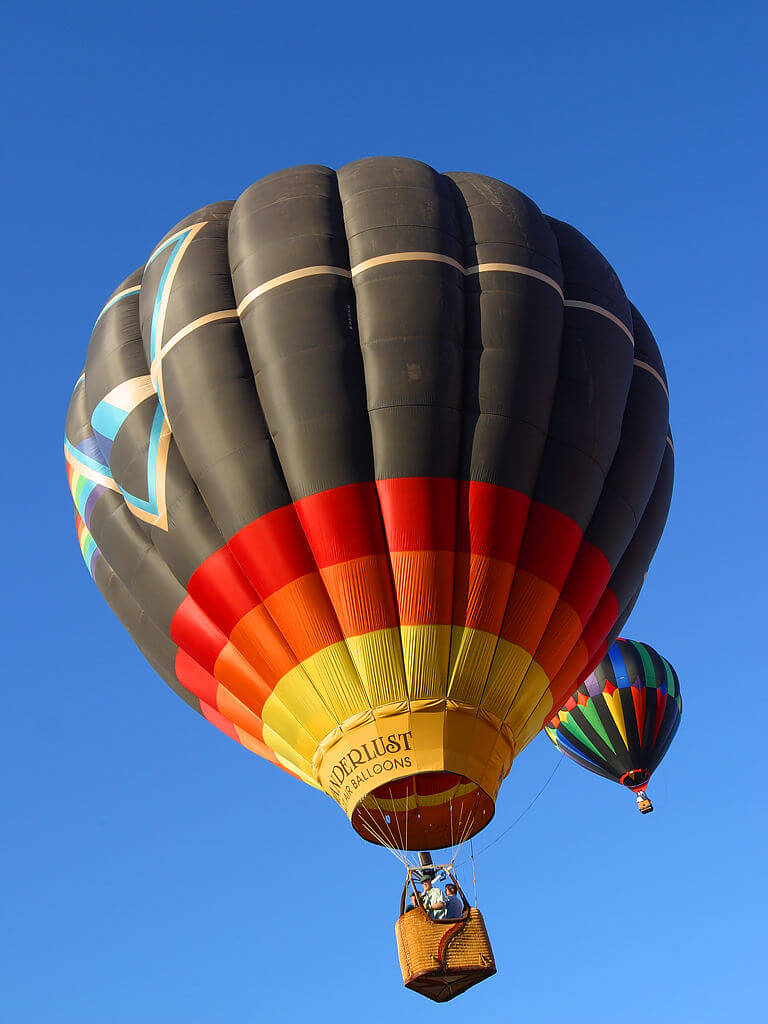
\includegraphics[width=0.4\textwidth]{01-EtudeAeronefs/img/montgolfiere.jpg}
  	\legende{2 ballons dirigeables}{img:montgolfiere}
	\end{figure}	
	
	\histoire{La montgolfière a été le premier aéronef conçu par l'humain. Les frères Montgolfier ont conçu le premier ballon à air chaud et réalisé le premier vol en 1783. La même année, ils font voler des animaux puis Jean-François \textbf{Pilâtre de Rozier} et le Marquis d'Arlandes réalisent le premier vol libre humain. \\ \\ En 1785, Jean-Pierre Blanchard effectue la première traversée de la manche avec un aéronef, 124 ans avant celle effectuée par Louis Blériot en avion.}
	\subsubsection{Ballon à gaz}
	Le ballon à gaz \anglais{gas balloon} est gonflé avec un gaz plus léger que l'air (hydrogène ou hélium).	
	
	\subsubsection{Dirigeable}
	Le dirigeable \anglais{airship} ou ballon dirigeable est un ballon à gaz équipé de systèmes propulsifs lui permettant de se diriger (aussi bien sur le plan horizontal que vertical). \\
	
	Les premiers dirigeables étaient gonflés à l'hydrogène. Ce gaz est dangereux car très inflammable. Les dirigeables modernes sont désormais gonflés à l'hélium. L'hélium est un gaz sûr car ininflammable, mais il est plus cher et plus lourd que l'hydrogène (un ballon à l'hélium nécessitera une enveloppe plus grande qu'un ballon à hydrogène de même capacité).
	
	\info{Il existe également des dirigeables à air chaud.}
	
	\begin{figure}[H]
  	\centering
    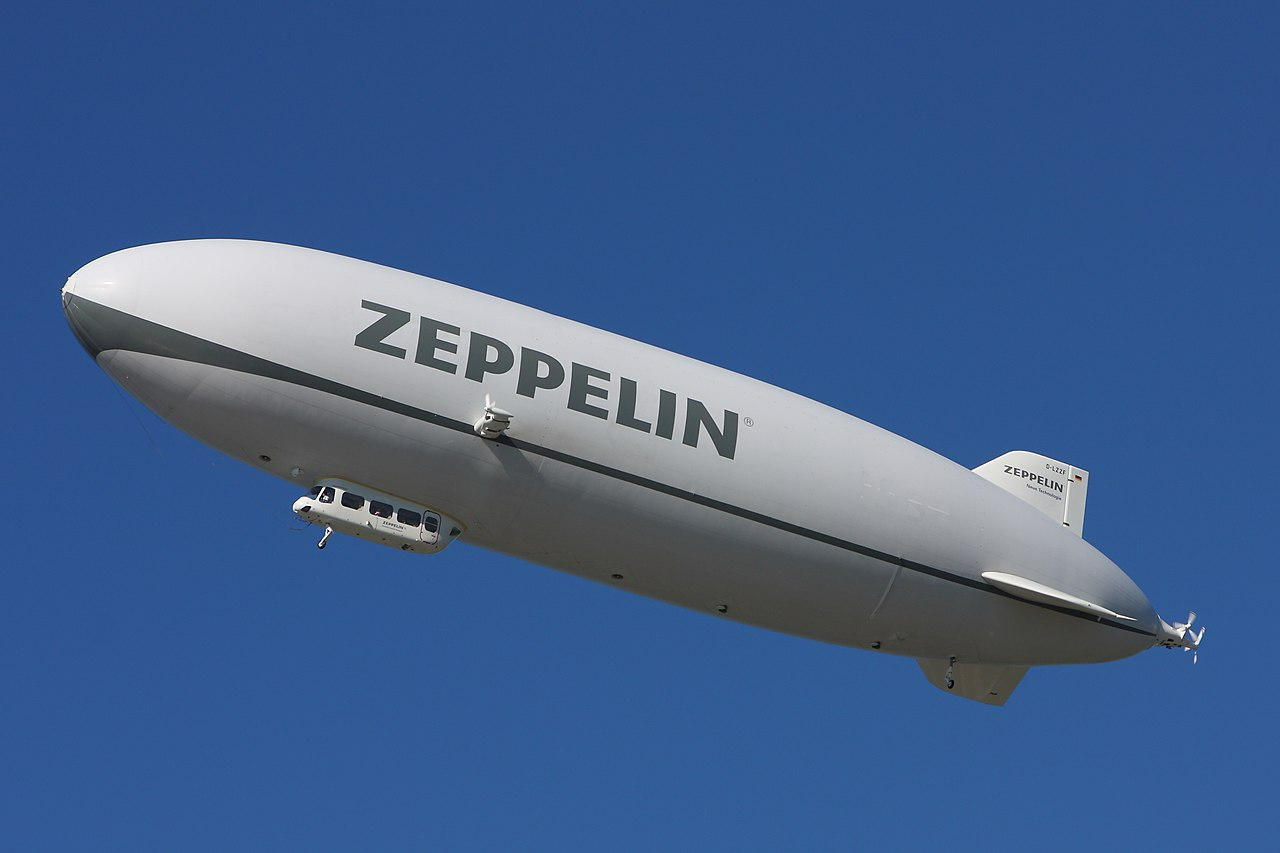
\includegraphics[width=0.4\textwidth]{01-EtudeAeronefs/img/dirigeable.jpg}
  	\legende{Un dirigeable moderne}{img:dirigeable}
	\end{figure}	

\subsection{Aérodynes}
	\subsubsection{Aéronef à voilure fixe}
		Les appareils à voilure fixe \anglais{fixed-wing aircraft}, également appelés aéroplanes sont des aéronefs dont la sustentation est assurée grâce à des phénomènes aérodynamiques sur des surfaces fixes (ailes). Ce type d'aéronef ne peut se maintenir en l'air que si un flux d'air suffisant existe sur ses surfaces portantes.

		\paragraph{Avions}
		La mise en mouvement de l'avion \anglais{airplane} est assuré par son ou ses moteurs. \\
		
		Il existe une très grande diversité de modèles d'avions, variables en taille, vitesse, conception et usages. \\
		
		\histoire{En France, Clément Ader aurait fait voler son Éole dès 1890, mais il n'existe pas de preuve formelle que cet appareil était effectivement quitté le sol. \\ \\  Le premier vol attesté d'un aérodyne à moteur a été réalisé par les frères Wright en 1903 aux États-Unis. C'est cette date qui est officiellement retenue comme celle du premier vol d'un avion.}
	
		\paragraph{Planeurs}
		Le planeur \anglais{glider} est un aérodyne dépourvu de moyens de propulsion. Il est donc dépendant de moyens annexes (remorqueur, treuil) pour sa mise en l'air. \\
		
		Une fois en l'air, le planeur peut exploiter des phénomènes atmosphériques pour gagner de l'altitude. \\
		
		\info{Il existe également des modèles de planeurs équipés de moteurs. Appelés motoplaneurs, ces planeurs peuvent généralement décoller de façon autonome.}
		
		\histoire{Le premier aérodyne à avoir volé est un planeur. Ce vol historique a été réalisé en 1891 par 	\textbf{Otto Lilienthal}.}
		
	\subsubsection{Aéronef à voilure tournante}
	Les appareils à voilure tournante \anglais{rotary-wing aircraft}, également appelés aérogires, sont des aéronefs dont la sustentation est assurée par la rotation d'un ou plusieurs rotors.
	
		\paragraph{Hélicoptères}
		L'hélicoptère \anglais{helicopter} est un aérodyne dont la sustentation est assurée grâce à un rotor entrainé par un moteur.
		
		Les inventeurs qui ont cherché à concevoir les premières hélicoptères au début du \siecle{20} cherchaient à concevoir une machine plus souple que les appareils à voilure fixe en permettant un décollage court voir vertical. 
		
		\histoire{L'idée de la machine à voilure tournante n'est pas récente, puisque l'on dispose de dessins du Léonard de Vinci datés du \siecle{15} représentant des machines à voilures tournantes.}
		
		\paragraph{Autogire}
		L'autogire \anglais{autogyro} est un aérodyne dont la sustentation est assurée grâce à un rotor entrainé par le vent relatif. Les autogires doivent donc dispose d'un mode de propulsion (typiquement une hélice entrainée par un moteur à pistons) qui assure la propulsion de l'appareil sur le plan horizontal.
		
		\histoire{L'autogire à précédé l'hélicoptère. Le premier vol d'un autogire a été effectué en 1923, contre 1936 pour le premier vol réellement contrôlé pour un hélicoptère.}
		
		\paragraph{Convertible}
		Les convertibles \anglais{tiltrotor } sont en quelque sort des hybrides entre des appareils à voilure tournante et des appareils à voilure fixe.
		
		Grâce à des systèmes qui permettent à leurs rotors de basculer d'une position verticale à une position horizontale, ces appareils cherchent à combiner les avantages de l'hélicoptère (vol stationnaire, décollage et atterrissage verticaux) à ceux des appareils à voilure fixe (vitesse de croisière). Cela se fait cependant au prix d'une complexité technique qui rend l'exploitation de ces appareils couteuse et délicate.
		
	\begin{figure}[H]
  	\centering
    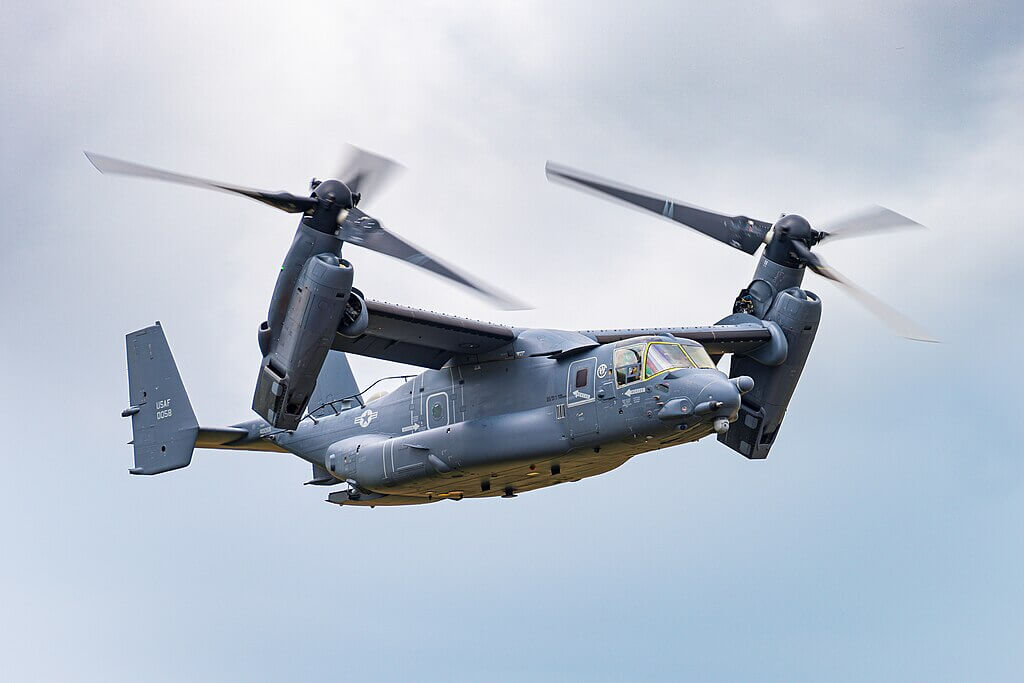
\includegraphics[width=0.4\textwidth]{01-EtudeAeronefs/img/tiltrotor.jpg}
  	\legende{Un convertible : le V22 Osprey}{img:tiltrotor}
	\end{figure}	
		
	\subsubsection{Aéronef à voilure souple}
	Les aéronefs à voilure souple \anglais{flexible wings} regroupent des aéronefs dont la voilure est généralement gonflée par l'air : parapente, paramoteur, parachute sportif moderne... Les deltaplanes rentrent également dans cette catégorie.
	
	\info{Le parachute, dans sa version initiale (coupole), se trouve à a limite de la définition d'un aéronef. En effet, ce type de parachute ne produit pas de portance (uniquement de la traînée) et sa capacité de manœuvre est très limitée.}
	
	\begin{figure}[H]
	\begin{minipage}[c]{0.35\linewidth}
	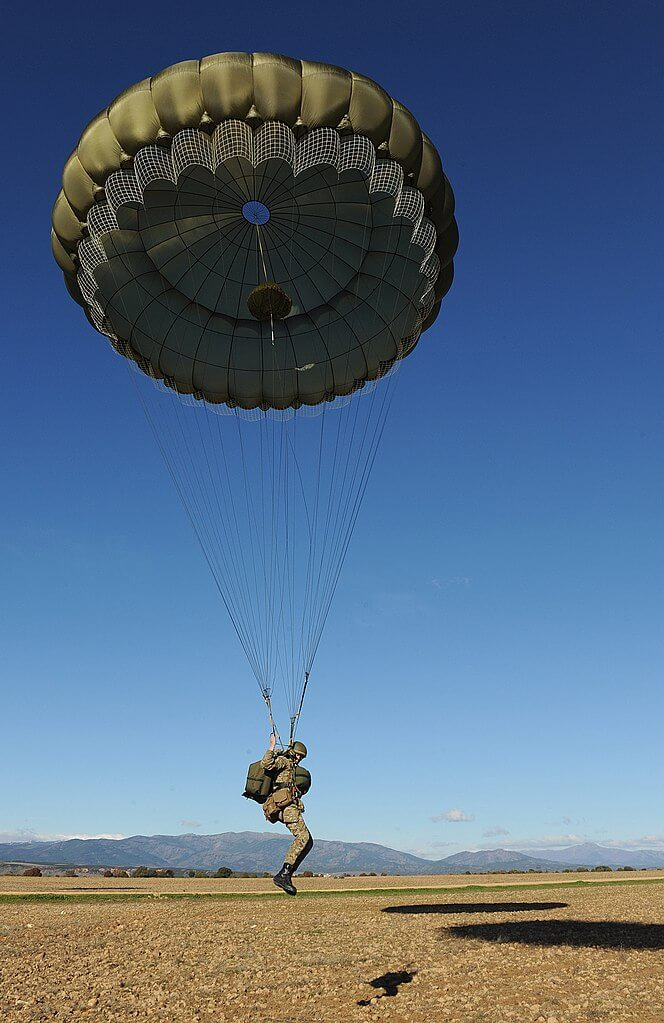
\includegraphics[width=\linewidth]{01-EtudeAeronefs/img/paraMili.jpg}
	\legende{Un parachute coupole}{img:paraMili}
	\end{minipage}
	\hfill
	\begin{minipage}[c]{0.35\linewidth}
	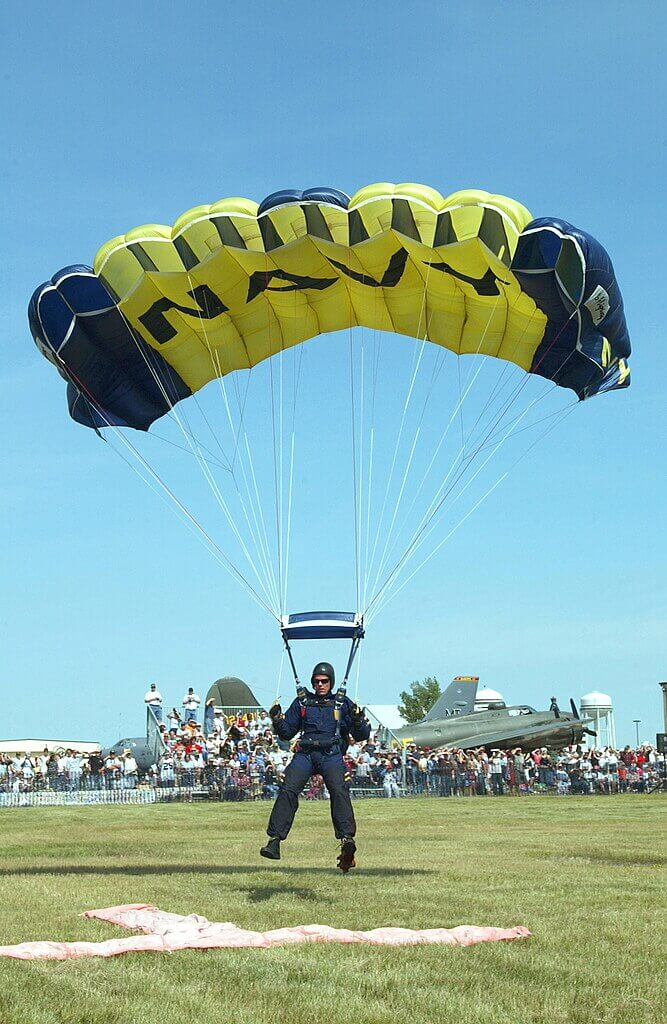
\includegraphics[width=\linewidth]{01-EtudeAeronefs/img/paraSport.jpg}
	\legende{Un parachute sportif moderne}{img:paraSport}
	\end{minipage}
	\end{figure}
	
	\histoire{André-Jacques \textbf{Garnerin}, un ingénieur français, effectue le premier saut réussi en parachute en 1797, en sautant depuis un ballon au dessus de Paris.}
	
\subsection{Engins spatiaux}
	\subsubsection{Lanceurs}
		\paragraph{Fusées}
		\paragraph{Navettes spatiales}
		
	\subsubsection{Engins spatiaux}
		\paragraph{Satellites}
		\paragraph{Sondes}

\subsection{Des grandes familles d'aéronefs}		
\subsubsection{Les ULM}

Les \acrshort{ulm} (\acrlong{ulm}) \anglais{ultralight aircraft} sont un ensemble d'aéronefs motorisés de faible masse. De par cette caractéristique, ils bénéficient de facilités quant à leurs conditions de conception et d'entretien. L'obtention d'une licence de pilote ULM est également simplifiée par rapport aux licences pour des appareils plus lourds (une licence ULM peut s'obtenir après environ 20h de vol). \\

Il existe une grande diversité d'ULM. Il est ainsi possible de piloter des ULM aérostats ou aérondynes, à voilures fixes, tournantes ou souples. En France, ils sont classés en 6 catégories. La licence de pilote d'ULM est commune à toutes les classes, cependant, il faut obtenir une qualification propre à chaque classe, qui permet au pilote de se familiariser avec un instructeur aux particularités propre à chaque type d'aéronef. \\

Chaque classe dispose de ses propres limitations en termes de masse et puissance maximale. Les ULM sont monoplace ou biplace.

	\paragraph{Classe 1 : paramoteur}

	Cette classe est composée d'aérodynes à voilure souple. Elle prend la forme d'un voile type voile de parapente. Le système propulsif, composé d'un moteur et d'une hélice carénée, est soit porté directement dans le dos par le pilote, soit fixé sur un chariot.  
	
	\begin{figure}[H]
  	\centering
    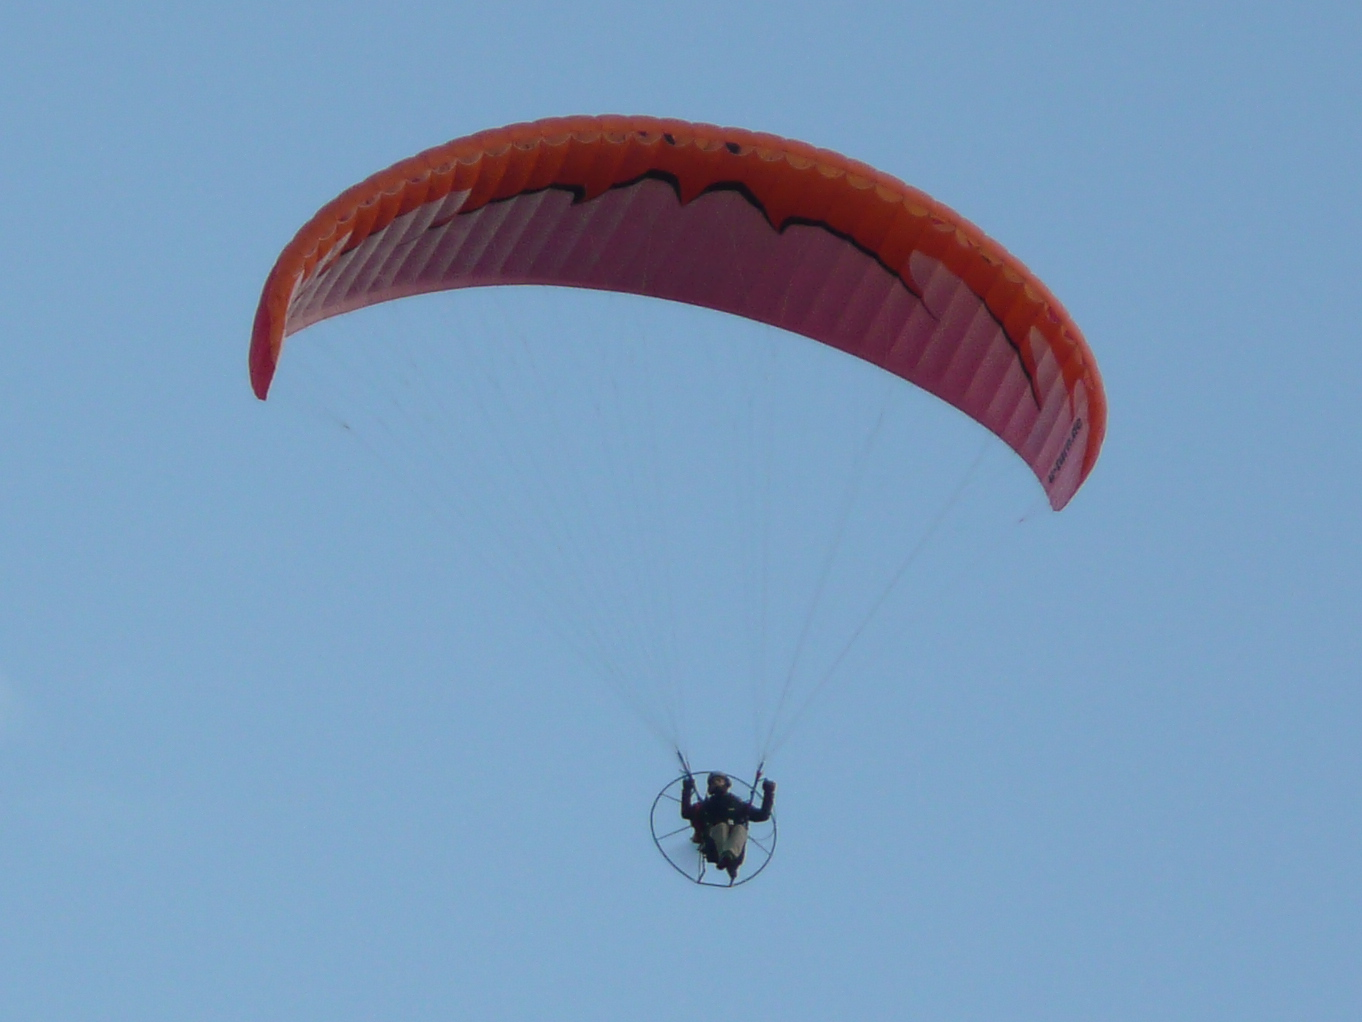
\includegraphics[width=0.4\textwidth]{01-EtudeAeronefs/img/ULM_Classe_1.jpg}
  	\legende{ULM classe 1}{img:ulmClasse1}
	\end{figure}	
	
	\paragraph{Classe 2 : pendulaire}
	Cette classe est composée d'aérodynes constitués de chariots sur lequel est fixé une aile delta. Le nom pendulaire vient du fait que les changements de trajectoires sont obtenus par déplacement du centre de gravité.	
	
	\begin{figure}[H]
  	\centering
    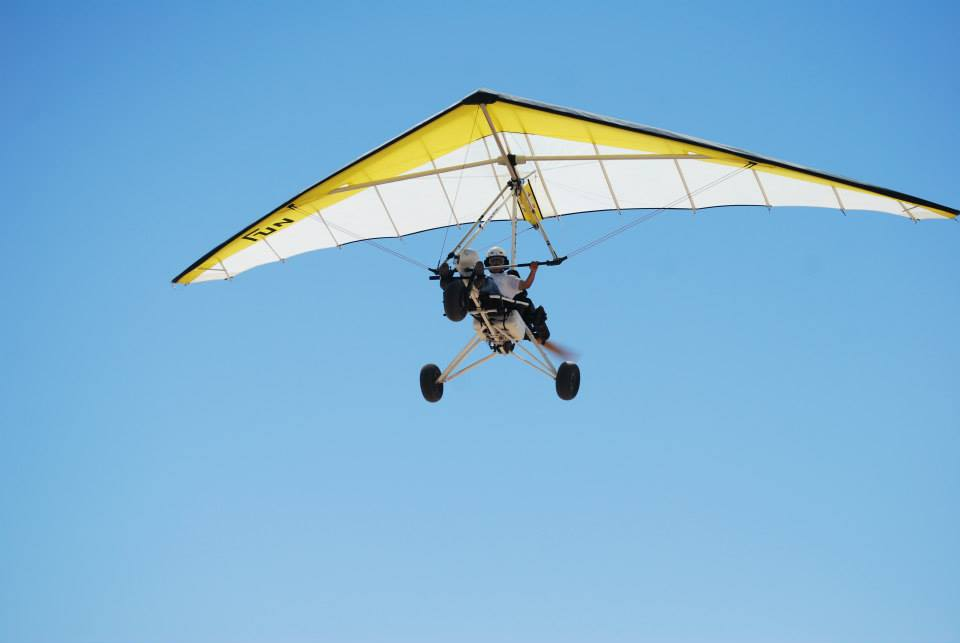
\includegraphics[width=0.4\textwidth]{01-EtudeAeronefs/img/ULM_Classe_2.jpg}
  	\legende{ULM classe 2}{img:ulmClasse2}
	\end{figure}	

	\paragraph{Classe 3 : multiaxes}
	Cette classe est composée d'aérodynes à voilure fixe, qui s'apparentent à des avions traditionnels. Ils est par ailleurs parfois difficile de distinguer un ULM  multiaxe moderne d'un avion biplace.
	
	\info{Aujourd'hui la frontière entre avion et ULM mutliaxes est très réduite. A un telle point que certains fabricants d'avion proposent un même modèle sous la réglementation avion ou ULM en fonction de la masse maximale inscrite sur les documents. C'est le cas de l'ULM présenté en photo ci dessous (commercialisé sous le nom Bristell Classic sous réglementation ULM et Bristel B23 en réglementation avion).}
	
	\begin{figure}[H]
  	\centering
    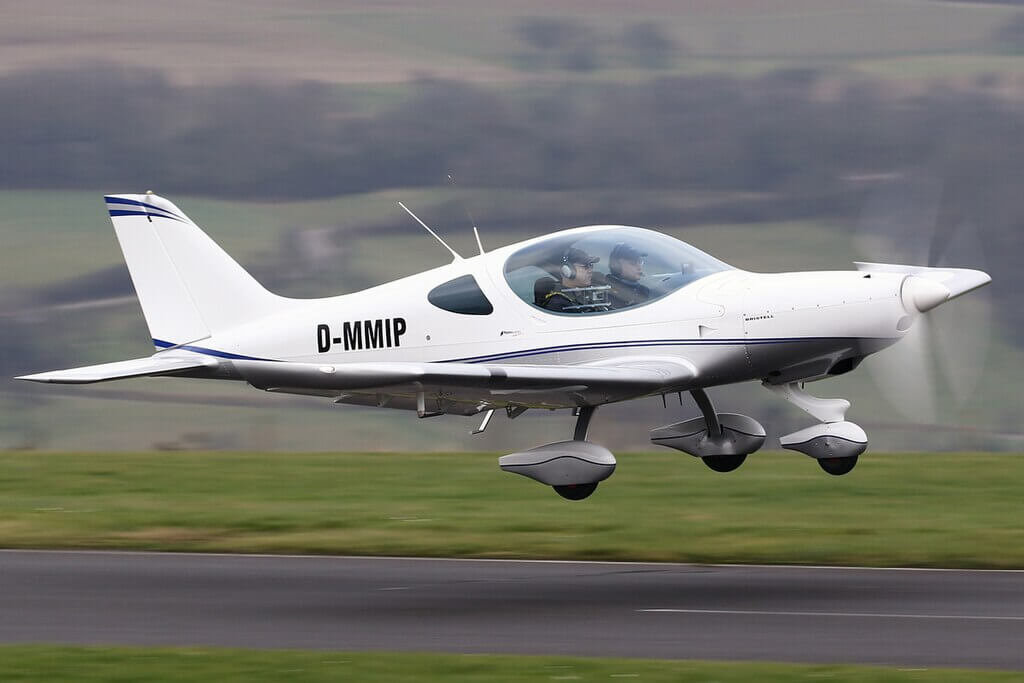
\includegraphics[width=0.4\textwidth]{01-EtudeAeronefs/img/ULM_Classe_3.jpg}
  	\legende{ULM classe 3}{img:ulmClasse3}
	\end{figure}	

	\paragraph{Classe 4 : autogyre}
	Cette classe est composée d'aérodynes à voilure tournante de type autogyres.

	\begin{figure}[H]
  	\centering
    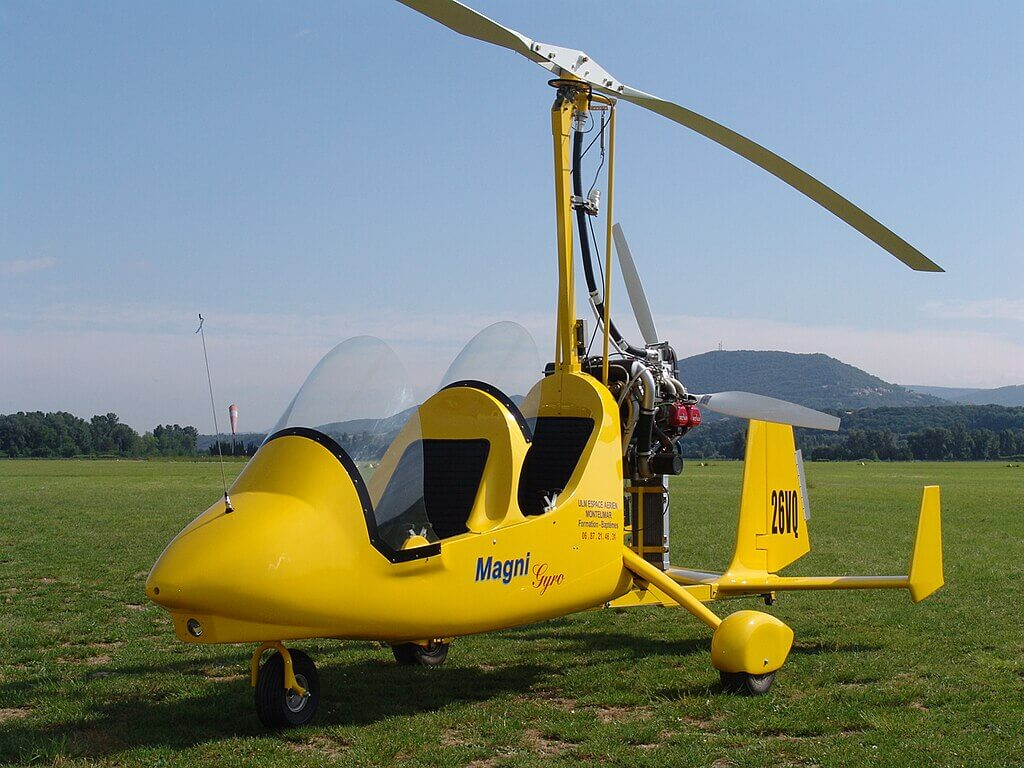
\includegraphics[width=0.4\textwidth]{01-EtudeAeronefs/img/ULM_Classe_4.jpg}
  	\legende{ULM classe 4}{img:ulmClasse4}
	\end{figure}	
	
	\paragraph{Classe 5 : ballon dirigeable}
	Il s'agit d'aérostats dirigeables dont le volume de l'enveloppe est inférieur à 900 m² pour un  ballon à l'hélium et 2000 m² pour les ballons à air chaud.	
	
	\begin{figure}[H]
  	\centering
    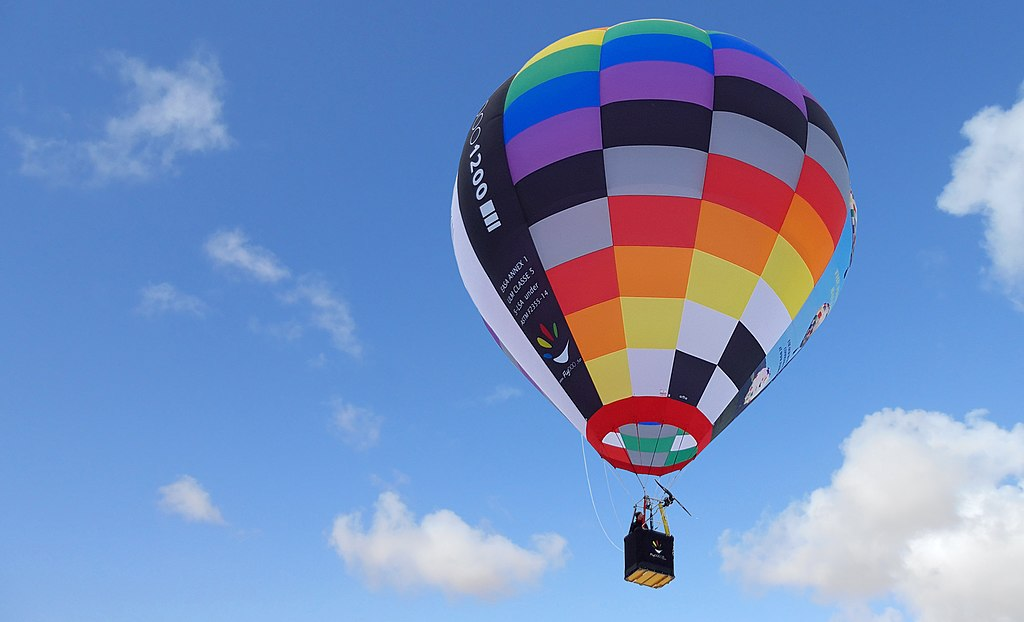
\includegraphics[width=0.4\textwidth]{01-EtudeAeronefs/img/ULM_Classe_5.jpg}
  	\legende{ULM classe 5}{img:ulmClasse5}
	\end{figure}	
		
	\paragraph{Classe 6 : hélicoptère}	
	Dernière née des catégories d'ULM (créer en 2012), cette classe est composée d'aérodynes à voilure tournante de type hélicoptères.
	
	\begin{figure}[H]
  	\centering
    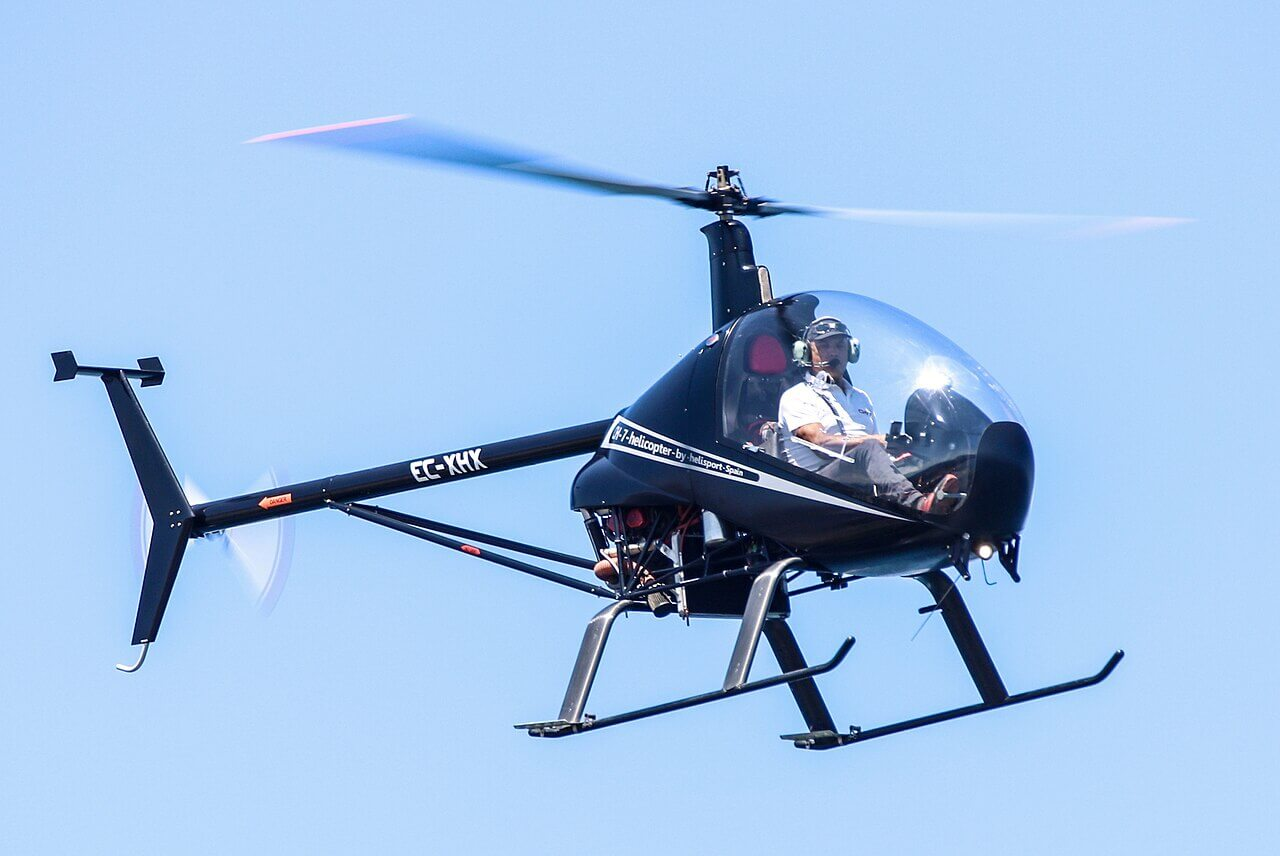
\includegraphics[width=0.4\textwidth]{01-EtudeAeronefs/img/ULM_Classe_6.jpg}
  	\legende{ULM classe 6}{img:ulmClasse6}
	\end{figure}


\subsubsection{Les drones}
Les drones sont des aéronefs pilotés à distance. 

Les drones peuvent être tout type d'aéronef : voilure tournante (typiquement multirotors), voilure fixe, aérostat... Les drones peuvent être libres ou captifs (retenus au sol par un câble).

Il existe également une grande diversité dans les dimensions du drones. Cela va d'appareils mesurant quelques dizaines de centimètre de côté et quelques centaines de grammes à des machines de plusieurs tonnes et de grande envergure. \\

Un système drone est toujours composé de systèmes au sol permettant le contrôle du drone ainsi que du drone lui même. Le drone doit comporter de nombreux systèmes pour assurer son autonomie énergétique, le contrôle de son attitude, le contrôle de sa trajectoire et le suivi de son plan de vol ou encore la liaison dans les 2 sens avec le système de pilotage à distance. 

Enfin, il faut ajouter à ces systèmes les systèmes propres à la mission du drone : capteurs (photo, infrarouge, radio...), systèmes de largage ou d'épandage...

		\usetikzlibrary{calc,fit}
\tikzset{>=latex} % for LaTeX arrow head
\colorlet{knob}{blue!20!black!40}
\colorlet{mylightblue}{blue!10}
\colorlet{mydarkblue}{blue!30!black}
\tikzstyle{arrow}=[<-,very thick,mydarkblue]
\tikzstyle{vector}=[->,line width=2,green!50!black]

% ANGLE
\newcommand{\getangle}[3]{%
    \pgfmathanglebetweenpoints{\pgfpointanchor{#2}{center}}
                              {\pgfpointanchor{#3}{center}}
    \global\let#1\pgfmathresult  
}

\newcommand{\echelleTikz}{1.0}

% ENGINE
\def\gas{blue!10}
\def\engine#1{
  \def\R{2}
  \def\l{1}
  \def\L{4.6}
  \def\p{1.8}
  \def\P{3.2}
  \def\Ra{.35} % crankshaft
  \def\Rb{.6}  % crankshaft
  \def\Rc{.2}  % crankshaft
  \def\a{40} % wall
  \def\b{30} % rod
  \coordinate (O)   at (0,0);
  \coordinate (CS)  at (#1:\l);
  \coordinate (P)   at (0,{\l*sin(#1)+sqrt(\P^2-(\l*cos(#1))^2)});
  \coordinate (RL)  at (180-\a:\R);
  \coordinate (RR)  at (\a:\R);
  \coordinate (TL)  at ($(RL)+(0,\L)$);
  \coordinate (TR)  at ($(RR)+(0,\L)$);
  \coordinate (T)   at ($(TL)!.5!(TR)$);
  \coordinate (PL)  at ($(RL)+(0,{\l*(1.4+sin(#1))})$);
  
  \coordinate (PR)  at ($(PL-|RR)+(0,\p)$);
  \coordinate (S)   at ($(T)+(0,.8)$);
  \coordinate (VLo) at ($(TL)!.2!(S)$);
  \coordinate (VL)  at ($(TL)!.4!(S)$);
  \coordinate (VLm) at ($(TL)!.6!(S)$);
  \coordinate (VRo) at ($(TR)!.2!(S)$);
  \coordinate (VR)  at ($(TR)!.4!(S)$);
  \coordinate (VRm) at ($(TR)!.6!(S)$);
  \getangle{\c}{CS}{P}
  \getangle{\vl}{VLo}{VLm}
  \getangle{\vr}{VRo}{VRm}
  
  % GAS
  \fill[\gas,draw=white,line width=3] (PL) -| (TR) -- (S) -- (TL) -- cycle;
  
  % CRANKSHAFT
  \draw[thick,mydarkblue,top color=blue!30!black!40,bottom color=blue!30!black!10,shading angle=180]
    (O) ++ (180+#1:\Ra) to[out={-90+#1},in={180+#1},looseness=.8]
    ($(CS)+(-90+#1:\Rb)$) arc (-90+#1:90+#1:\Rb) to[out=180+#1,in=90+#1,looseness=.8] cycle;
  
  % ROD
  \draw[thick,mydarkblue,top color=blue!30!black!50,bottom color=blue!30!black!20,shading angle=\c]
    (CS) ++ (\c-\b:\Rb) arc (\c-\b:-360+\c+\b:\Rb) -- ($(P)+(\c+90:\Rc)$) -- ($(P)+(\c-90:\Rc)$) -- cycle;
  
  % PISTON
  \draw[mydarkblue,thick,top color=blue!20!black!30,bottom color=blue!20!black!30,middle color=blue!5,shading angle=90]
    (PL) rectangle (PR);
  \draw[thick,mydarkblue,fill=knob]
    (PL) ++ (0,.65*\p) rectangle ($(PR)+(0,-.25*\p)$);
  
  % DECORATION
  \draw[thick,mydarkblue,fill=knob] (O) circle (\Rc/2);
  \draw[thick,mydarkblue,fill=knob] (CS) circle (\Rc);
  \draw[thick,mydarkblue,fill=knob] (P) circle (\Rc);
  
  % WALL
  \wall
}

% WALL
\def\wall{
  \draw[line width=4,blue!10!black!50]
    (VRo) ++ (1.5,0.6) to[out=180,in=60] (VRo) -- (TR) -- %to[out=-30,in=90,looseness=0.5]
    (RR) arc (\a:-180-\a:\R) --
    (TL) -- (VLo) to[out=110,in=0] ++ (-1.5,0.6); %to[out=90,in=200,looseness=0.8]
  \draw[line width=4,blue!10!black!50]
    (VLo) ++ (-1.5,1.3) to[out=0,in=110] (VLm) -- (S) --
    (VRm) to[out=60,in=180] ($(VRo)+(1.5,1.3)$);
    
  \fill[blue!30!black!60]
    (S) ++ (.07,.2) to[out=90,in=-150]++ (1,1.4) -- ($(S)+(1,1.74)$)
    to[out=-150,in=90] ($(S)+(-.07,.2)$);
  \draw[blue!30!black!80]
    (S) ++ (.07,.2) to[out=90,in=-150]++ (1,1.4)
    (S) ++ (-.07,.2) to[out=90,in=-150]++ (1.07,1.54);
  \draw[blue!10!black,fill=blue!20!black]
    (S) ++ (-.09,-.16) --++ (.09,-.1) coordinate (X) --++ (.09,.1) -- cycle;
  \draw[blue!30!black,fill=blue!30!black!80]
    (S) ++ (-.1,-.15) --++ (.2,0) --++ (0,.35) --++ (-.2,0) -- cycle;
}

% VALVE
\def\valveL#1{
  \fill[thick,blue!20!black]
    (VLo) ++ (\vl-90:#1) -- ($(VLm)+(\vl-90:#1)$) -- ($(VLo)!.64!(VLm)+(\vl+90:.2-#1)$) --++ (\vl+90:2)
    -- ($(VLo)!.36!(VLm)+(\vl+90:2.2-#1)$) -- ($(VLo)!.36!(VLm)+(\vl+90:.2-#1)$) -- cycle;
}

% VALVE
\def\valveR#1{
  \fill[thick,blue!20!black]
    (VRo) ++ (\vr+90:#1) -- ($(VRm)+(\vr+90:#1)$) -- ($(VRo)!.64!(VRm)+(\vr-90:.2-#1)$) --++ (\vr-90:2)
    -- ($(VRo)!.36!(VRm)+(\vr-90:2.2-#1)$) -- ($(VRo)!.36!(VRm)+(\vr-90:.2-#1)$) -- cycle;
}

\section{Les groupes motopropulseurs}

	\subsection{Moteurs à pistons}
		\subsubsection{Description du moteur à piston}
		Le moteur à piston, également appelé moteur à combustion interne ou moteur à explosion est un moteur qui transforme l'énergie chimique contenue dans le carburant (essence, gasoil, gaz...) en énergie mécanique.
		\begin{figure}[H]
  		\centering
    		% INTAKE STROKE
\def\gas{blue!50}
\resizebox{\echelleTikz\width}{\echelleTikz\height}{
\begin{tikzpicture}
  \def\d{-60}
  \engine{10};
  \draw[vector] (\d:.6*\R) arc (\d:\d-80:.55*\R);
  \fill[\gas, opacity=0.5]
    (VLo) to[out=110,in=0] ++ (-1.5,0.6) -- ($(VLo)+(-1.5,1.3)$) to[out=0,in=110] (VLm) to[out=\vl+5,in=\vl-47] cycle;
  \wall
  \valveL{.3}
  \valveR{.1}
  
  \draw[arrow] (VL) ++ (-.2,.2) --++ (-1,-.5)
    node[below left=-2,align=right,scale=1.4] {valve\\[-2pt]d'admission};
  \draw[arrow] (VR) ++ (.2,.1) --++ (1,-.5)
    node[below right=-2,align=left,scale=1.4] {valve\\[-2pt]d'échappement};
  \draw[arrow] (O) ++ (-.2,.4) --++ (-2.0,.9)
    node[left=-20,above left=2,scale=1.4] {villebrequin};
  \draw[arrow] (P) ++ (1.1,-.2) --++ (1.2,-.5)
    node[below right=-2,scale=1.4] {piston};
  \draw[arrow] (P) ++ (1.5,0.4) --++ (1.2,-.5)
    node[below right=-2,scale=1.4] {cylindre};
  \draw[arrow] (P) ++ (-1,0.97) --++ (-1.2,-.5);
  \draw[arrow] (P) ++ (-1,0.67) --++ (-1.2,-.2) %-0.5 - (0.97-0.67) = -0.2
    node[below left=-2,scale=1.4] {segments};
  \draw[arrow] (PL) ++ (2.2,-1.9) --++ (1.68,-.7)
    node[below right=-2,scale=1.4] {bielle};
  \draw[arrow] (O) ++ (-1.9,-0.8) --++ (-1.2,.5)
    node[left=-20,above left=2,scale=1.4] {carter};
  \draw[arrow] (S) ++ (150:.2) --++ (-.5,.7)
    node[above=-1,align=center,scale=1.4] {bougie};
  \draw[arrow] (VLm) ++ (-1.5,.5) --++ (-1.5,.7)
    node[above left=-2,align=right,scale=1.4] {pipe\\[-2pt]d'admission};
  \draw[arrow] (VRm) ++ (1.5,.5) --++ (1.5,.7)
    node[above right=-2,align=left,scale=1.4] {pipe\\[-2pt]d'échappement};
  
\end{tikzpicture}
}
  		\legende{Schéma d'un moteur à piston}{tikz::schemaMoteurPiston}
		\end{figure}
		
		Le moteur à piston est composé des éléments principaux suivants :
		\begin{itemize}
			\item cylindre
			\item piston : pièce mobile dans le cylindre
			\item bielle : pièce qui fait la jonction entre le cylindre et le vilebrequin
			\item vilebrequin : manivelle qui convertit le mouvement alternatif du piston en mouvement rotatif
			\item bougie : système d'allumage qui permet de commander la combustion du mélange contenu dans le cylindre
			\item soupape d'admission et d'échappement : pièces mobiles qui permettent de faire rentrer le mélange et de faire sortir les gaz d'échappement du cylindre 
			\item pipe d'admission et d'échappement : tubes qui permettent d'acheminer respectivement le mélange air-essence dans le réservoir et les gaz brûlés vers l'échappement
			\item carter : bas du moteur. Contient notamment l'huile nécessaire au fonctionnement du moteur
			\item segment : anneau métallique installé sur le cylindre. Assure l'étanchéité entre le piston et le cylindre.
		\end{itemize}
	
		\subsubsection{Le cycle à 4 temps}
		\renewcommand{\echelleTikz}{0.5}
		\paragraph{Admission}
		
		L'admission est le premier cycle du cycle à 4 temps. Durant cette phase, qui démarre alors que le piston est en point haut, la soupape d'admission s'ouvre. La descente du piston durant cette étape permet l'aspiration du mélange air-carburant dans le cylindre. Lorsque le cylindre atteint son point bas, la soupape d'admission est refermée.

		\begin{figure}[H]
  		\centering
    		% INTAKE STROKE
\def\gas{blue!50}
\begin{tikzpicture}[scale=\echelleTikz]
  \def\d{-60}
  \engine{10};
  %\draw[vector] (\d:.6*\R) arc (\d:\d-80:.55*\R);
  \fill[\gas, opacity=0.5]
    (VLo) to[out=110,in=0] ++ (-1.5,0.6) -- ($(VLo)+(-1.5,1.3)$) to[out=0,in=110] (VLm) to[out=\vl+5,in=\vl-47] cycle;
  \wall
  \valveL{.3}
  \valveR{.1};
  
\end{tikzpicture}
  		\legende{Étape 1 : Admission}{tikz::schemaMoteurPiston}
		\end{figure}	

		\paragraph{Compression}
		
		Dans ce deuxième cycle, qui débute alors que le piston est en position basse, les 2 soupapes sont fermées. Le piston remonte et le mélange air-carburant précédemment admis est comprimé dans le cylindre.
		
		\begin{figure}[H]
  		\centering
    		% COMPRESSION STROKE
\def\gas{blue!50}
\begin{tikzpicture}[scale=\echelleTikz]
  \def\d{-10}
  \engine{-140};
  \draw[vector] (\d:.6*\R) arc (\d:\d-80:.55*\R);
  \valveL{.1}
  \valveR{.1}
\end{tikzpicture}
  		\legende{Étape 2 : Compression}{tikz::schemaMoteurPiston}
		\end{figure}	
		
		\paragraph{Explosion-détente}
		
		Dans ce cycle, qui démarre alors que le piston atteint à nouveau le point haut, l'étincelle provoquée par la bougie provoque l'explosion du mélange présent dans le cylindre. Le piston est alors repoussé vers le bas. Durant ce cycle, les 2 soupapes restent fermées.
		
		\begin{figure}[H]
  		\centering
		% IGNITION
\def\gas{blue!50}
\resizebox{\echelleTikz\width}{\echelleTikz\height}{
\begin{tikzpicture}
  \def\d{40}
  \engine{90};
  \draw[vector] (\d:.6*\R) arc (\d:\d-80:.55*\R);
  \valveL{.1}
  \valveR{.1}
  \draw[very thin,yellow!70!black,fill=yellow,shift={(X)}]
    ( -15:.20) -- ( -30:.40) -- ( -40:.25) -- ( -50:.40) --
    ( -60:.22) -- ( -70:.40) -- ( -80:.20) -- ( -90:.45) --
    (-100:.24) -- (-110:.40) -- (-120:.25) -- (-130:.40) --
    (-140:.20) -- (-150:.45) -- (-165:.20) to[out=40,in=140] cycle;
\end{tikzpicture}
}
  		\legende{Étape 3 : Explosion-détente}{tikz::schemaMoteurPiston}
		\end{figure}	
		
		\info{Le cycle d'explosion-détente est le seul cycle qui produit effectivement de l'énergie.}
		
		\paragraph{Échappement}
		
		Dans cette quatrième et dernière étape du cycle, la soupape d'échappement est ouverte. Le piston, initialement en point bas, remonte et pousse les gaz brûlés issus de la combustion en dehors du cylindre lors de la remontée. L'étape d'échappement se termine lorsque le piston atteint le point haut, la soupape d'échappement est alors refermée.
		
		\begin{figure}[H]
  		\centering
		% EXHAUST STROKE
\def\gas{blue!50}
\resizebox{\echelleTikz\width}{\echelleTikz\height}{
\begin{tikzpicture}
  \def\d{-40}
  \engine{-190};
  \draw[vector] (\d:.6*\R) arc (\d:\d-80:.55*\R);
  \fill[\gas, opacity=0.5]
    (VRo) to[out=60,in=-180] ++ (1.5,0.6) -- ($(VRo)+(1.5,1.3)$) to[out=180,in=60] (VRm) to[out=-220+\vr,in=-180+\vr] cycle;
  \wall
  \valveL{.1}
  \valveR{.3}
\end{tikzpicture}
}
  		\legende{Étape 4 : Échappement}{tikz::schemaMoteurPiston}
		\end{figure}	
		
		\paragraph{Cycle complet}
		
		L'animation suivante permet de visualiser le fonctionnement d'un moteur à explosion.	
		
		\renewcommand{\echelleTikz}{0.5}
		\begin{figure}[H]
  		\centering
		\begin{animateinline}[autoplay,loop,controls]{60}
 \multiframe{360}{i=-90+2}{
    \begin{tikzpicture}
	  \coordinate (boiteLegende1) at (0,8.5);
    	  \coordinate (boiteLegende2) at (0,9);
      \node[rectangle,minimum width=2cm] [fit = (boiteLegende1) (boiteLegende2)] (legende) {};    
    
      %\def\d{-10}
      \engine{-\i};
      %\draw[vector] (\d:.6*\R) arc (\d:\d-80:.55*\R);
      %\valveL{.1}
      %\valveR{.1}

	% INTAKE STROKE
	\ifnum\i>-92 \ifnum\i<-88 
	    \node[align=center,font=\Large] at (legende.center) {\textbf{Admission}};
		\valveL{.2}
  		\valveR{.1} ;
	\fi \fi 
	\ifnum\i>-90 \ifnum\i<90 
	    \node[align=center,font=\Large] at (legende.center) {\textbf{Admission}};
		\fill[\gas]
    		(VLo) to[out=110,in=0] ++ (-1.5,0.6) -- ($(VLo)+(-1.5,1.3)$) to[out=0,in=110] (VLm) to[out=\vl-90,in=\vl-90] cycle;
  		\wall
		\valveL{.3}
  		\valveR{.1} ;
	\fi \fi
	\ifnum\i>88 \ifnum\i<92 
	    \node[align=center,font=\Large] at (legende.center) {\textbf{Admission}};
		\valveL{.2}
  		\valveR{.1} ;
	\fi \fi 
	% COMPRESSION STROKE
	\ifnum\i>90 \ifnum\i<272 
	    \node[align=center,font=\Large] at (legende.center) {\textbf{Compression}};
		\valveL{.1}
  		\valveR{.1} ;
	\fi \fi 
	% POWER STROKE
	\ifnum\i>270 \ifnum\i<452 
		\node[align=center,font=\Large] at (legende.center) {\textbf{Explosion-détente}};
		\valveL{.1}
  		\valveR{.1} ;
	\fi \fi
	% EXHAUST STROKE
	\ifnum\i>450 \ifnum\i<454
	    \node[align=center,font=\Large] at (legende.center) {\textbf{Echappement}};
		\valveL{.1}
  		\valveR{.2} ;
	\fi \fi
	\ifnum\i>452 \ifnum\i<630
	    \node[align=center,font=\Large] at (legende.center) {\textbf{Echappement}};
		\fill[\gas]
    		(VRo) to[out=60,in=-180] ++ (1.5,0.6) -- ($(VRo)+(1.5,1.3)$) to[out=180,in=60] (VRm) to[out=-270+\vr,in=-270+\vr] cycle;
  		\wall 
		\valveL{.1}
  		\valveR{.3} ;
	\fi \fi
	\ifnum\i>630 \ifnum\i<632
	    \node[align=center,font=\Large] at (legende.center) {\textbf{Echappement}};
		\valveL{.1}
  		\valveR{.2} ;
	\fi \fi

	% IGNITION
	\ifnum\i>268 \ifnum\i<280 
		\draw[very thin,yellow!70!black,fill=yellow,shift={(X)}]
    		( -15:.20) -- ( -30:.40) -- ( -40:.25) -- ( -50:.40) --
    		( -60:.22) -- ( -70:.40) -- ( -80:.20) -- ( -90:.45) --
    		(-100:.24) -- (-110:.40) -- (-120:.25) -- (-130:.40) --
   	 	(-140:.20) -- (-150:.45) -- (-165:.20) to[out=40,in=140] cycle; 
	\fi \fi 

      
    \end{tikzpicture}
  }
\end{animateinline}
  		\legende{Le fonctionnement d'un moteur à explosion (animé)}{tikz::schemaMoteurPistonAnime}
		\end{figure}	
		
	\subsubsection{Nombre et disposition des cylindres}
	Pour augmenter la puissance et la régularité de fonctionnement, la plupart des moteurs à pistons sont dôtés de plusieurs cylindres. Ce nombre va de 1 à 28 cylindres pour les plus gros moteurs.
	
	Dans l'histoire des moteurs à pistons, les concepteurs de ces moteurs ont testé de nombreuses dispositions. Chacune a ses forces et ses faiblesses, nous listerons ici quelques unes des dispositions les plus courantes parmi les dispositions que l'on trouve dans l'aéronautique.
	
	\paragraph{Cylindres en ligne}
	
	\paragraph{Moteur à plat}
	
	\paragraph{Moteur en étoile}
	Le moteur en étoile \anglais{radial engine} a été très utilisée dans l'aviation. En effet, il présente de nombreux avantages dans une utilisation aéronautique :
	\begin{itemize}
		\item refroidissement : tous les cylindres sont exposés de façon identique au flux d'air de refroidissement
		\item compacité et légèreté
		\item système de graissage naturellement adapté à une utilisation "toute position" et donc à la voltige
	\end{itemize}
	
	\info{Les moteurs en étoile sont toujours équipés d'un nombre impair de cylindres.}
	
	\paragraph{Moteur en V}
	
	\subsection{Motorisation électrique}
	
	\subsection{Turbopropulseurs et turbomoteurs}
	\begin{figure}[H]
  	\centering
    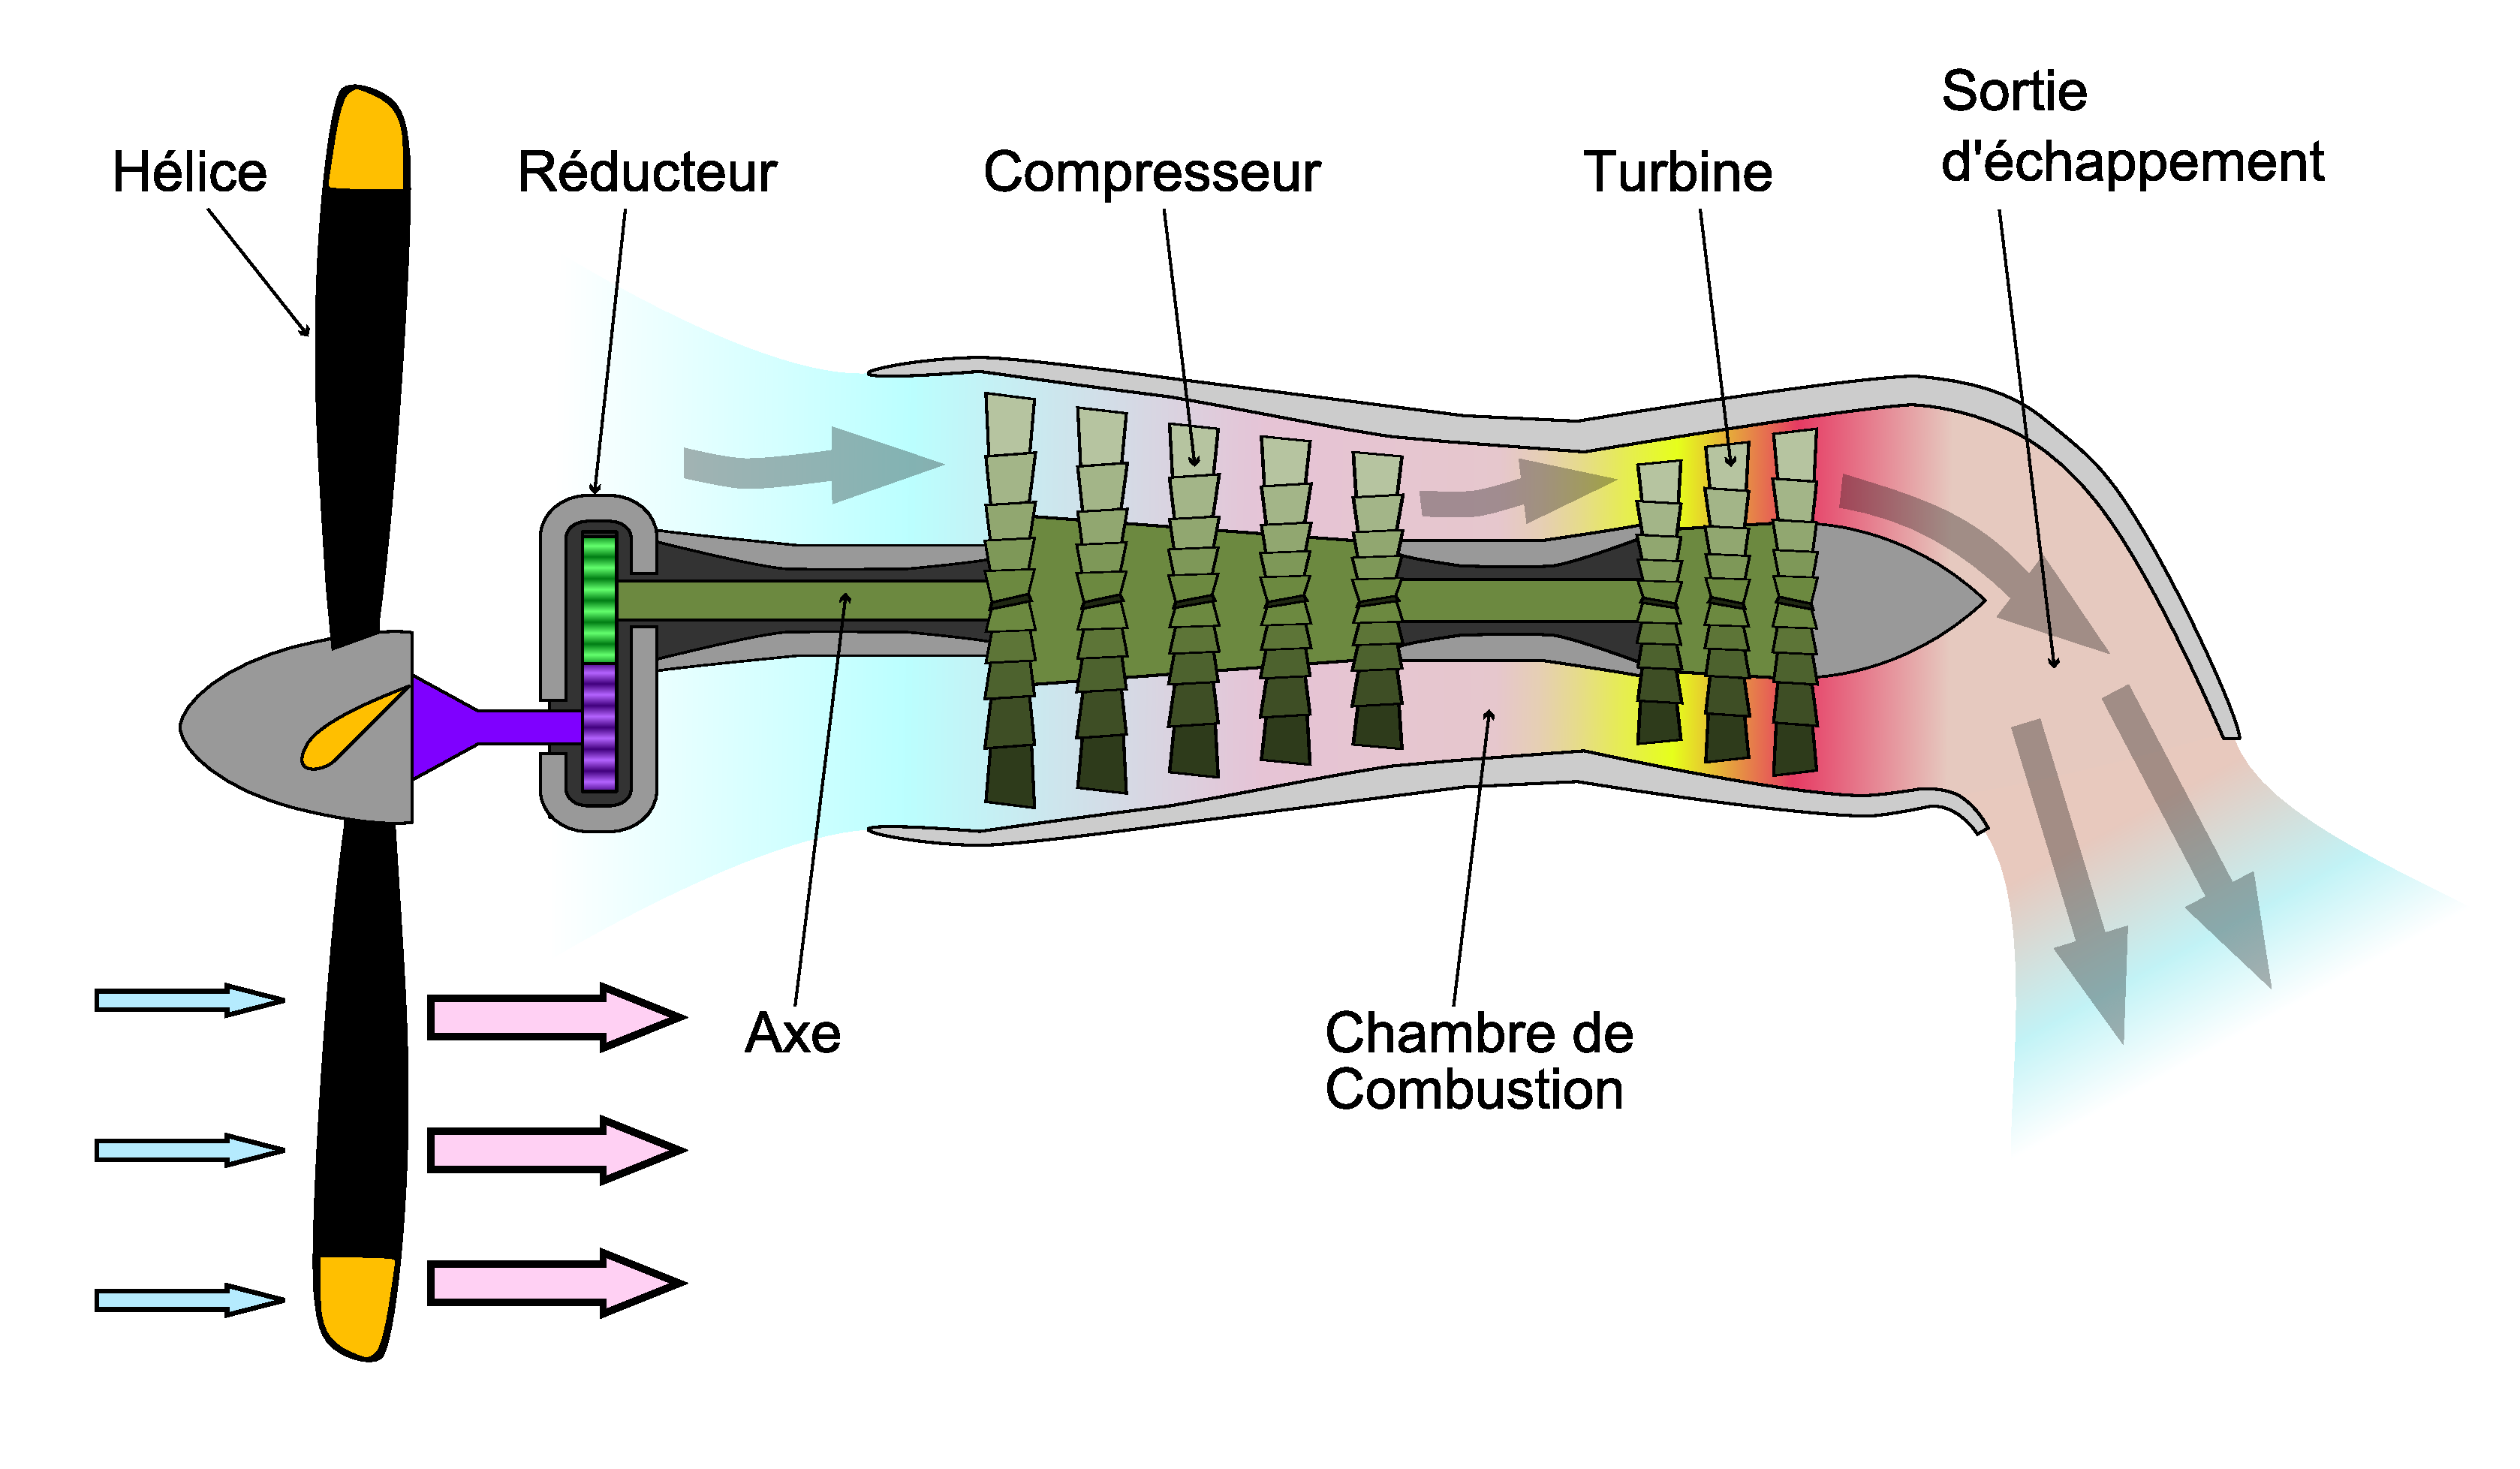
\includegraphics[width=0.75\textwidth]{01-EtudeAeronefs/img/turbomachines/turbopropulseur.pdf}
  	\legende{Schéma d'un turbopropulseur}{img:turbopropulseur}
	\end{figure}	
	
	\subsection{Hélices et moteurs}
	
	\subsection{Propulseurs à réaction}
		\subsubsection{Turboréacteurs}
		
		\begin{figure}[H]
  		\centering
    		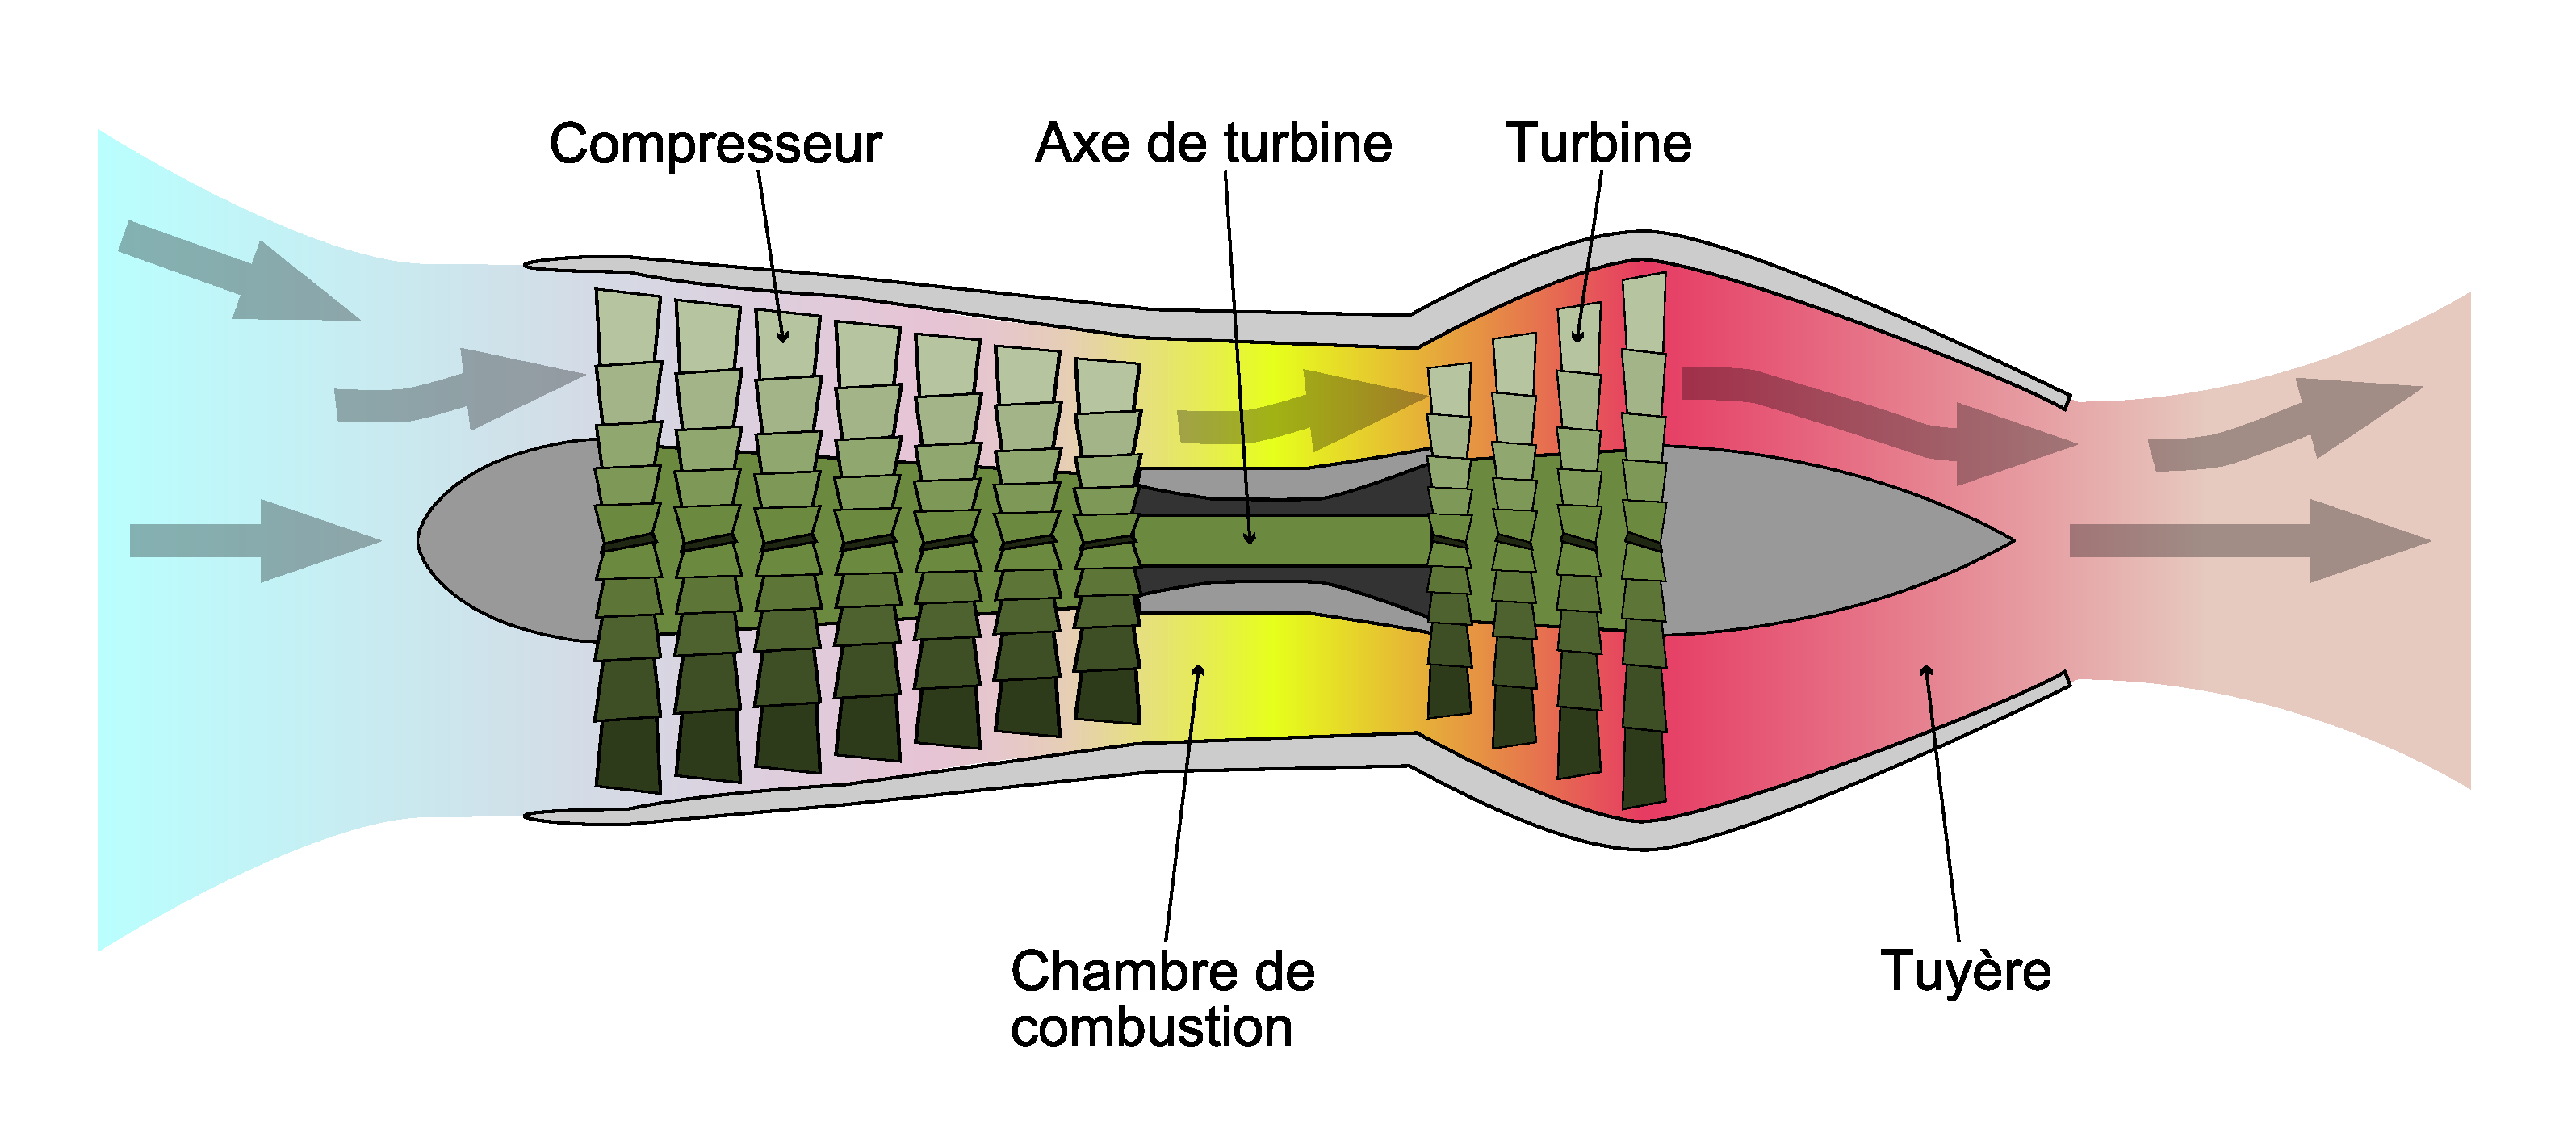
\includegraphics[width=0.75\textwidth]{01-EtudeAeronefs/img/turbomachines/turboreacteur-simpleFlux.pdf}
  		\legende{Schéma d'un turboréacteurs simple flux}{img:turboreacteur-simpleFlux}
		\end{figure}	
	
		\begin{figure}[H]
  		\centering
    		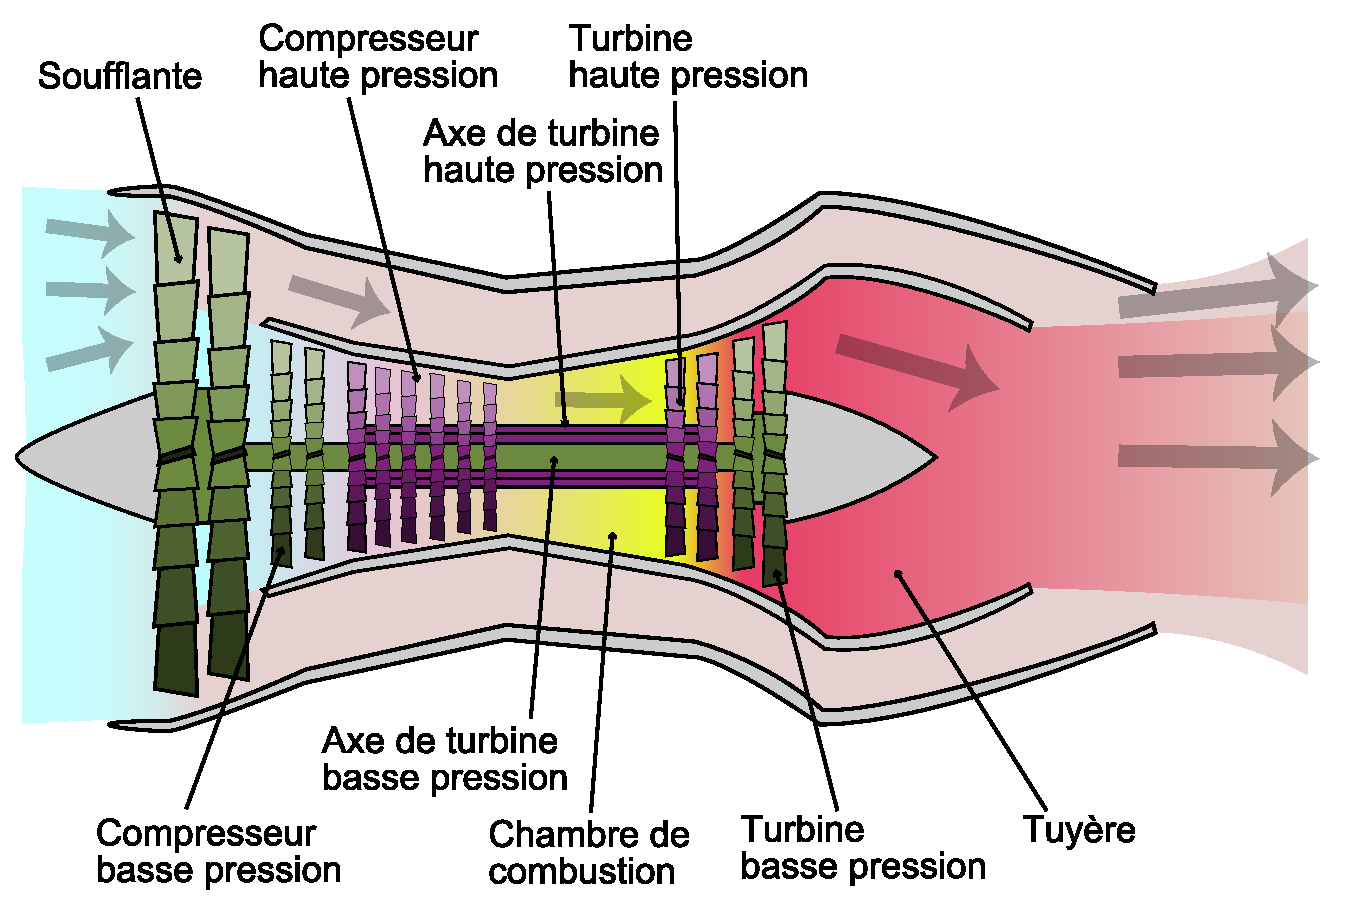
\includegraphics[width=0.75\textwidth]{01-EtudeAeronefs/img/turbomachines/turboreacteur-doubeFlux.pdf}
  		\legende{Schéma d'un turboréacteurs double flux}{img:turboreacteur-doubeFlux}
		\end{figure}	
	
		\subsubsection{Statoréacteurs}
	
		\subsubsection{Moteurs fusées}
		
	\subsection{Contraintes liées au développement durable}

		\section{Structures et matériaux}
		\section{Les commandes de vol}
		%éléments communalisés
\pgfdeclareimage{case}{01-EtudeAeronefs/img/instruments/alt/alt_case.pdf}

\pgfdeclareimage{asiFace}{01-EtudeAeronefs/img/instruments/asi/asi_face.pdf}
\pgfdeclareimage{asiHand}{01-EtudeAeronefs/img/instruments/asi/asi_hand.pdf}
\pgfdeclareimage{asiCase}{01-EtudeAeronefs/img/instruments/asi/asi_case.pdf}

\pgfdeclareimage{altCase}{01-EtudeAeronefs/img/instruments/alt/alt_case.pdf}
\pgfdeclareimage{altFace1}{01-EtudeAeronefs/img/instruments/alt/alt_face_1.pdf}
\pgfdeclareimage{altFace2}{01-EtudeAeronefs/img/instruments/alt/alt_face_2.pdf}
\pgfdeclareimage{altFace3}{01-EtudeAeronefs/img/instruments/alt/alt_face_3.pdf}
\pgfdeclareimage{altHand1}{01-EtudeAeronefs/img/instruments/alt/alt_hand_1.pdf}
\pgfdeclareimage{altHand2}{01-EtudeAeronefs/img/instruments/alt/alt_hand_2.pdf}

\pgfdeclareimage{aiCase}{01-EtudeAeronefs/img/instruments/ai/ai_case.pdf}
\pgfdeclareimage{aiFace}{01-EtudeAeronefs/img/instruments/ai/ai_face.pdf}
\pgfdeclareimage{aiRing}{01-EtudeAeronefs/img/instruments/ai/ai_ring.pdf}
\pgfdeclareimage{aiBack}{01-EtudeAeronefs/img/instruments/ai/ai_back.pdf}

\pgfdeclareimage{hiCase}{01-EtudeAeronefs/img/instruments/hi/hi_case.pdf}
\pgfdeclareimage{hiFace}{01-EtudeAeronefs/img/instruments/hi/hi_face.pdf}

\pgfdeclareimage{tcCase}{01-EtudeAeronefs/img/instruments/tc/tc_case.pdf}
\pgfdeclareimage{tcFace1}{01-EtudeAeronefs/img/instruments/tc/tc_face_1.pdf}
\pgfdeclareimage{tcFace2}{01-EtudeAeronefs/img/instruments/tc/tc_face_2.pdf}
\pgfdeclareimage{tcBall}{01-EtudeAeronefs/img/instruments/tc/tc_ball.pdf}
\pgfdeclareimage{tcBack}{01-EtudeAeronefs/img/instruments/tc/tc_back.pdf}
\pgfdeclareimage{tcMark}{01-EtudeAeronefs/img/instruments/tc/tc_mark.pdf}

\pgfdeclareimage{vsiCase}{01-EtudeAeronefs/img/instruments/vsi/vsi_case.pdf}
\pgfdeclareimage{vsiHand}{01-EtudeAeronefs/img/instruments/vsi/vsi_hand.pdf}
\pgfdeclareimage{vsiFace}{01-EtudeAeronefs/img/instruments/vsi/vsi_face.pdf}

\pgfdeclareimage{ilsCase}{01-EtudeAeronefs/img/instruments/ils/ils_case.pdf}
\pgfdeclareimage{ilsCaseFixed}{01-EtudeAeronefs/img/instruments/ils/ils_case_fixed.pdf}
\pgfdeclareimage{ilsFace}{01-EtudeAeronefs/img/instruments/ils/ils_face.pdf}
\pgfdeclareimage{ilsFlagGs}{01-EtudeAeronefs/img/instruments/ils/ils_flag_gs.pdf}
\pgfdeclareimage{ilsFlagNav}{01-EtudeAeronefs/img/instruments/ils/ils_flag_nav.pdf}
\pgfdeclareimage{ilsHandGs}{01-EtudeAeronefs/img/instruments/ils/ils_hand_gs.pdf}
\pgfdeclareimage{ilsHanvNav}{01-EtudeAeronefs/img/instruments/ils/ils_hand_nav.pdf}

%altimètre
%   -paramètre 1 : altitude en pieds
%   -paramètre 2 : calage en pouces de mercure
\def\alti#1#2{
	\fill[transparent] (0,0) circle (3) ;
	\node[rotate=(#2-28.0)*100] {\pgfbox[center,center]{\pgfuseimage{altFace1}}};
	\node {\pgfbox[center,center]{\pgfuseimage{altFace2}}};
  	\node[rotate=-{(Mod(#1/10,10000))*(36/1000)}] {\pgfbox[center,center]{\pgfuseimage{altFace3}}};
  	\node[rotate=-{(Mod(#1,1000))*(360/1000)}] {\pgfbox[center,center]{\pgfuseimage{altHand2}}};
    	\node[rotate=-{(Mod(#1,10000))*(360/10000)}] {\pgfbox[center,center]{\pgfuseimage{altHand1}}};
    	%\node {\pgfbox[center,center]{\pgfuseimage{altCase}}};
	\node {\pgfbox[center,center]{\pgfuseimage{case}}};
}

%consevateur de cap
%   -paramètre 1 : cap en degrés
\def\conservateurCap#1{
	\fill[transparent] (0,0) circle (3) ;
  	\node[rotate=#1] {\pgfbox[center,center]{\pgfuseimage{hiFace}}};
    	\node {\pgfbox[center,center]{\pgfuseimage{hiCase}}};
}

%ILS
%   -paramètre 1 : QDM en degrés
%   -paramètre 2 : décallage horizontal
%   -paramètre 3 : décallage vertical
\def\ils#1#2#3{
	\fill[transparent] (0,0) circle (3) ;
		\node {\pgfbox[center,center]{\pgfuseimage{ilsCaseFixed}}};
		\node {\pgfbox[center,center]{\pgfuseimage{ilsFlagGs}}};
		\node {\pgfbox[center,center]{\pgfuseimage{ilsFlagNav}}};
		\node[yshift=-#2*32] {\pgfbox[center,center]{\pgfuseimage{ilsHandGs}}};
		\node[xshift=-#2*32] {\pgfbox[center,center]{\pgfuseimage{ilsHanvNav}}};
		\node[rotate=#1] {\pgfbox[center,center]{\pgfuseimage{ilsFace}}};
    	\node {\pgfbox[center,center]{\pgfuseimage{ilsCase}}};
}

%variomètre
%   -paramètre 1 : taux de descente
\def\vario#1{
	\fill[transparent] (0,0) circle (3) ;
  	\node {\pgfbox[center,center]{\pgfuseimage{vsiFace}}};
   	\node[rotate=-(#1/2000)*172] {\pgfbox[center,center]{\pgfuseimage{vsiHand}}};
    	%\node {\pgfbox[center,center]{\pgfuseimage{vsiCase}}};
	\node {\pgfbox[center,center]{\pgfuseimage{case}}};
}

%horizon
%   -paramètre 1 : roulis
%   -parametre 2 : tangage 
\def\horizon#1#2{
	\fill[transparent] (0,0) circle (3) ;
	\node {\pgfbox[center,center]{\pgfuseimage{aiBack}}};
  	\node[rotate=#1,yshift=-#2*1.25] {\pgfbox[center,center]{\pgfuseimage{aiFace}}};
    	\node[rotate=#1] {\pgfbox[center,center]{\pgfuseimage{aiRing}}};
    	\node {\pgfbox[center,center]{\pgfuseimage{aiCase}}};
}

%indicateur de virage
%   -paramètre 1 : taux virage [-1;1] 
%   -parametre 2 : postion bille [-1;1] 
\def\indicateurVirage#1#2{
	\fill[transparent] (0,0) circle (3) ;
  	\node {\pgfbox[center,center]{\pgfuseimage{tcBack}}};
    	\node {\pgfbox[center,center]{\pgfuseimage{tcFace1}}};
    	\node {\pgfbox[center,center]{\pgfuseimage{tcFace2}}};
    	%\node[xshift=#2*35,yshift=#2*4] {\pgfbox[center,center]{\pgfuseimage{tcBall}}};
	\node[rotate around={#2*15:(0,3.7)}] {\pgfbox[center,center]{\pgfuseimage{tcBall}}};
    	\node[rotate=#1*20] {\pgfbox[center,center]{\pgfuseimage{tcMark}}};
    	%\node {\pgfbox[center,center]{\pgfuseimage{tcCase}}};
	\node {\pgfbox[center,center]{\pgfuseimage{case}}};
}

%badin
%   -paramètre 1 : vitesse [0;200] 
\def\badin#1{
	\fill[transparent] (0,0) circle (3) ;
  	\node {\pgfbox[center,center]{\pgfuseimage{asiFace}}};
    	
	%0 kts : 0°
	%40 kts : 36°
	%70 kts : 90°
	%130 kts : 210°
	%160 kts : 264°
	%200 kts : 312°

	%	Vitesse	Position aiguille	Angle/10 kts
	%	0		0,00°	
	%	40		36,00°		NA
	%	50		54,00°		-18°
	%	60		72,00°		-18°
	%	70		90,00°		-18°
	%	80		110,00°		-20°
	%	90		130,00°		-20°
	%	100		150,00°		-20°
	%	110		170,00°		-20°
	%	120		190,00°		-20°
	%	130		210,00°		-20°
	%	140		228,00°		-18°
	%	150		246,00°		-18°
	%	160		264,00°		-18°
	%	200		312,00°		-12°

	%Entre 0 et 40 kts
	\ifnum#1<41
	\node[rotate=-(((#1)/(40))*(36))] {\pgfbox[center,center]{\pgfuseimage{asiHand}}};
	\fi 
	%Entre 40 et 70 kts
	\ifnum#1>40 \ifnum#1<71
	\node[rotate=-(((#1-40)/(70-40))*(90-36))-36] {\pgfbox[center,center]{\pgfuseimage{asiHand}}};
	\fi \fi
	%Entre 71 et 130 kts
	\ifnum#1>70 \ifnum#1<131
	\node[rotate=-(((#1-70)/(130-70))*(210-90))-90] {\pgfbox[center,center]{\pgfuseimage{asiHand}}};
	\fi \fi
	%Entre 130 et 160 kts
	\ifnum#1>130 \ifnum#1<161
	\node[rotate=-(((#1-130)/(160-130))*(264-210))-210] {\pgfbox[center,center]{\pgfuseimage{asiHand}}};
	\fi \fi
	%Entre 160 et 200 kts
	\ifnum#1>160
	\node[rotate=-(((#1-160)/(200-160))*(312-264))-264] {\pgfbox[center,center]{\pgfuseimage{asiHand}}};
	\fi

    	%\node {\pgfbox[center,center]{\pgfuseimage{asiCase}}};
	\node {\pgfbox[center,center]{\pgfuseimage{case}}};
}

% Définir les clés pour les paramètres
\pgfkeys{
    /tdb/.is family,
    /tdb,
    vitesse/.store in = \tdbVitesse,
    altitude/.store in = \tdbAltitude,
    calageAltitude/.store in = \tdbCalageAltitude,
    vz/.store in = \tdbVz,
    cap/.store in = \tdbCap,
    assiette/.store in = \tdbAssiette,
    inclinaison/.store in = \tdbInclinaison,
    derapage/.store in = \tdbDerapage,
    virage/.store in = \tdbVirage,
    afficherT/.store in = \tdbAfficherT,
    vitesse = 0,
    altitude = 0,
    vz = 0,
    cap = 0,
    assiette = 0,
    inclinaison = 0,
    derapage = 0,
    virage = 0,
    calageAltitude = 30,
    afficherT = false,
}

% Nouvelle commande pour dessiner la planche de bord
\newcommand{\dessinerTdB}[1]{
    \pgfkeys{/tdb, #1}

    \begin{tikzpicture}
        % Définir les coordonnées des sommets de la planche de bord
        \coordinate (A) at (-5, 3.5);
        \coordinate (B) at (19, 3.5);
        \coordinate (C) at (19, -10.5);
        \coordinate (D) at (-5, -10.5);

        % Dessiner le polygone avec le coin supérieur gauche arrondi
        \fill[gray, rounded corners=3cm] (D) -- (A) -- (B) -- (C) -- cycle ;

        % Dessiner le polygone rouge si showredpolygon est vrai
        \ifthenelse{\equal{\tdbAfficherT}{true}}{
            \coordinate (T1) at (-3.2, 3.2);
            \coordinate (T2) at (17.2, 3.2);
            \coordinate (T3) at (17.2, -3.5);  
            \coordinate (T4) at (10.4, -3.5);
            \coordinate (T5) at (10.4, -10.2);
            \coordinate (T6) at (3.6, -10.2);
            \coordinate (T7) at (3.6, -3.5); 	
            \coordinate (T8) at (-3.2, -3.5); 
            \draw[line width=5pt, red] (T1) -- (T2) -- (T3) -- (T4) -- (T5) -- (T6) -- (T7) -- (T8) -- cycle  ;
        }{}

        % Placer les instruments
        \begin{scope}[xshift=0cm, yshift=0cm]
            \badin{\tdbVitesse}
        \end{scope}
        
        \begin{scope}[xshift=7cm, yshift=0cm]
            \horizon{\tdbInclinaison}{\tdbAssiette}
        \end{scope}
        
        \begin{scope}[xshift=14cm, yshift=0cm]
            \alti{\tdbAltitude}{\tdbCalageAltitude}
        \end{scope}
        
        \begin{scope}[xshift=0cm, yshift=-7cm]
            \indicateurVirage{\tdbVirage}{\tdbDerapage}
        \end{scope}
        
        \begin{scope}[xshift=7cm, yshift=-7cm]
            \conservateurCap{\tdbCap}
        \end{scope}
        
        \begin{scope}[xshift=14cm, yshift=-7cm]
            \vario{\tdbVz}
        \end{scope}

        %\draw (B) grid (D);    
        
    \end{tikzpicture}
}



\section{L'instrumentation de bord}
	\subsection{L'indicateur de vitesse}

	\begin{figure}[H]	
	\centering
	\begin{tikzpicture}
		\badin{110}
	\end{tikzpicture}
	%\caption[\cite{tikz::instrumentsBase}]{Un "badin"}
	%\caption{Un "badin" \cite{tikz::instrumentsBase}}
	\legende{Un "badin"}{tikz::instrumentsBase}
	\end{figure}
	
	\subsection{L'altimètre}
	
	\begin{figure}[H]	
	\centering
	\begin{tikzpicture}
		\alti{4500}{29.92}
	\end{tikzpicture}
	\legende{Un altimètre}{tikz::instrumentsBase}
	\end{figure}
	
	\subsection{L'horizon artificiel}
	
	\begin{figure}[H]	
	\centering
	\begin{tikzpicture}
		\horizon{0}{0}
	\end{tikzpicture}
	\legende{Un horizon artificiel}{tikz::instrumentsBase}
	\end{figure}
	
	\subsection{Le conservateur de cap}
	
	\begin{figure}[H]	
	\centering
	\begin{tikzpicture}
		\conservateurCap{83}
	\end{tikzpicture}
	\legende{Un conservateur de cap}{tikz::instrumentsBase}
	\end{figure}
	
	
	\subsection{L'indicateur de virage}
	
	\begin{figure}[H]	
	\centering
	\begin{tikzpicture}
		\indicateurVirage{0}{0}
	\end{tikzpicture}
	\legende{Un indicateur de virage}{tikz::instrumentsBase}
	\end{figure}
	
	
	\subsection{Le variomètre}
	
	\begin{figure}[H]	
	\centering
	\begin{tikzpicture}
	\vario{-500}
	\end{tikzpicture}
	\legende{Un variomètre}{tikz::instrumentsBase}
	\end{figure}
	
	\chapter{Navigation, réglementation, sécurité des vols}
	\label{nav}
		\section{Navigation}
	La navigation est une science qui permet de connaitre sa position sur la Terre, calculer la route à suivre pour atteindre une autre position, ou calculer toute autre information relativement au déplacement. \\

	Les techniques de navigation utilisées dans l'aéronautique sont reprises de celles alors utilisées dans la navigation maritime (avec, aux tous débuts de l'aviation l'utilisation de sextants pour s'orienter la nuit à partir des étoiles, puis la création de phares de navigation aérienne). Ces techniques permettaient de naviguer par temps clair, mais trouvaient rapidement leurs limites pour naviguer par conditions météo médiocres ou mauvaises.
	
	\begin{center}
	\begin{minipage}[c]{1.0\linewidth}
	\begin{figure}[H]
	\begin{minipage}[c]{0.4\linewidth}
	\centering
	\includegraphics[width=0.7\linewidth]{02-Navigation/img/Phare-aéronautique-de-Baziege.jpg}
	\legende{Le phare aéronautique de Baziège (construit en 1925)}{img:Phare-aéronautique-de-Baziege}
	\end{minipage}
	\begin{minipage}[c]{0.6\linewidth}
	\centering
	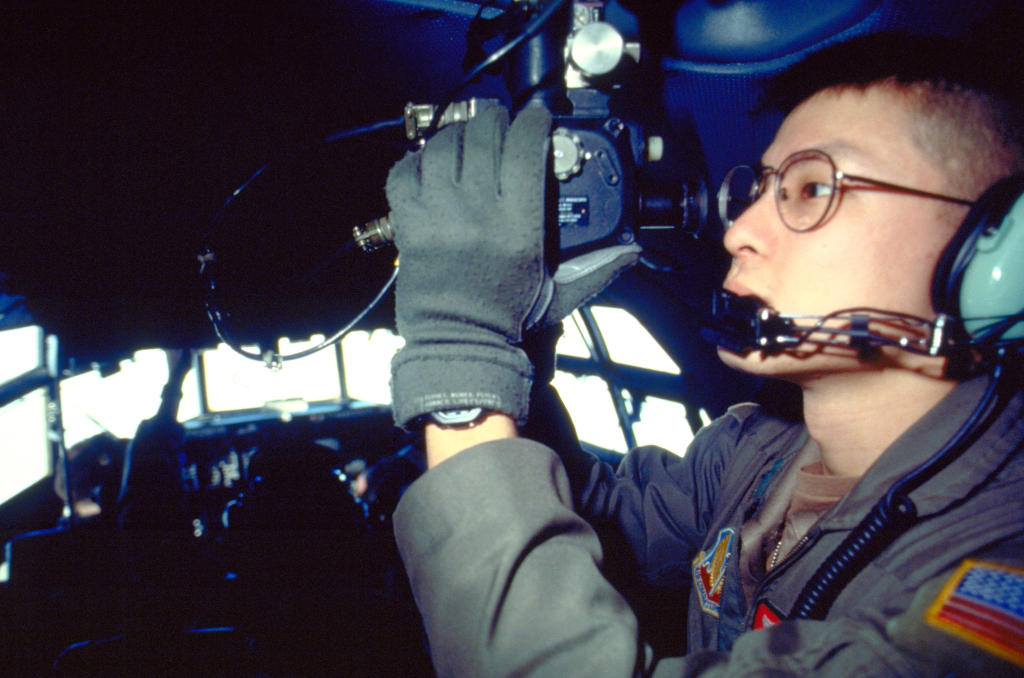
\includegraphics[width=0.95\linewidth]{02-Navigation/img/Sextant-C130.jpg}
	\legende{Utilisation d'un sextant dans un C130 (1996)}{img:Sextant-C130.jpg}
	\end{minipage}
	\end{figure}
	\end{minipage}
	\end{center}
	
	Peu à peu, les aviateurs ont donc développé des systèmes de radionavigation (NDB en 1920) qui utilisent des signaux radioélectriques plutôt que lumineux et visuels pour le repérage. Ces procédés de radionavigation fonctionnent de jour comme de nuit et sont utilisables par tous temps. Ces systèmes offrent aussi des portées bien supérieures à ceux des systèmes lumineux, ce qui permet alors d'envisager un maillage qui offre une couverture continentale. Ils nécessitent cependant des récepteurs embarqués dans les aéronefs pour être utilisables.
	
	Depuis les années 1970, la navigation aéronautique exploite de plus en plus les systèmes de navigation par satellite.\\
	
	Dans ce chapitre, nous allons étudier dans un premier temps quels sont les grands principes de la navigation aérienne, puis comment on se sert des systèmes de radionavigation.
	
	\subsection{Les grands principes de navigation}
		\subsubsection{Navigation à l'estime et cheminement à vue}
		\subsubsection{Route vraie, route magnétique, cap vrai, cap magnétique, déclinaison, déviation}
		\subsubsection{Distance entre deux points d'une carte}
		\subsubsection{Régimes de vol}
		Un aéronef évolue toujours selon des règles partagées. Pour les vols civils, on dit que l'on évolue selon les règles de la \textbf{\acrlong{cag}}	(\acrshort{cag}). La CAG défini 2 grandes régimes de vol : le VFR et l'IFR.\\
		
		Il existe d'autres règles de circulation aérienne, on peut citer par exemple la CAM (Circulation Aérienne Militaire) ou encore la CER (Circulation d'Essais et de Réception). Ces circulations ne seront pas abordées ici.
		
		\paragraph{Le vol à vue}
		Le vol \acrshort{vfr} (\anglais{\acrlong{oaci}} - règles de vol à vue) correspond historiquement au premier mode de navigation utilisé pour se déplacer en avion. Dans ce mode de navigation, on navigue principalement grâce à des repères au sol, et on pilote l'attitude de l'avion grâce a l'horizon naturel. 
		
		L'instrumentation minimale pour ce type de vol est très réduite. On peut naviguer aisément en VFR avec seulement un anémomètre (pour connaitre sa vitesse), une boussole (pour connaitre son cap) et une montre (pour mesurer le temps avant d'atteindre le prochain point de repère de la navigation), même si aujourd'hui les appareils exploités en VFR sont généralement équipés d'une instrumentation bien plus élaborée.
		
		\astuce{En français, on dit parfois VFR peut être traduit par \textbf{Voies-Ferrées/Routes} car pour naviguer selon les règles VFR on utilise des repères au sol, dont les routes et les voies ferrées.}
		
		Le principal inconvénient de ce mode de navigation est qu'il nécessite que les conditions météo soient suffisamment bonnes pour que l'horizon demeure visible et que les points de repères au sol soient identifiables. Ce régime de vol n'est donc utilisable que par beau temps. Les conditions de vols requises pour le vol VFR sont appelées \acrshort{vmc} (\anglais{\acrlong{vmc}} - conditions de vol à vue). Les conditions VMC définissent des visibilité horizontales et des distance par rapport aux nuages minimales permettant de voler à vue. Ces valeurs minimales dépendent de l'espace ou l'aéronef évolue.
		
		\info{Il est possible de voler selon les règles VFR la nuit, on parle alors de NVFR \anglais{Night VFR}.}
		
		\info{Il est possible de se servir des instruments de radionavigation ou du GPS pour naviguer en VFR, toujours en gardant les conditions VMC.}
		
		Aujourd'hui, ce mode de navigation reste très utilisée pour l'aviation de loisir mais également pour bon nombre de missions professionnelles (évacuations sanitaires, héliportage, surveillance d'infrastructures, largages de parachutistes...). \\
		
		Pour offrir des capacités de vol par conditions météo dégradées, il a donc fallu inventer un autre régime de vol : l'IFR.
		
		\paragraph{Le vol aux instruments}
		Le vol \acrshort{ifr} (\anglais{\acrlong{ifr}} - règles de vol aux instruments) définis les règles et procédure permettant de voler par tout temps, lorsque les conditions \acrshort{vmc} ne sont plus réunies. On se trouve alors en conditions \acrshort{imc}(\anglais{\acrlong{imc}} - conditions de vol aux instruments).
		
		Dans ces conditions, les informations visuelles obtenues par le sens du pilote (essentiellement la vue) ne permettent plus de piloter l'attitude de l'avion (absence d'horizon naturel) ni de naviguer (les repères au sol tout comme les obstacles sont cachés par la mauvaise visibilité, et deviennent invisibles ou visibles trop tardivement). Dans ces conditions, les pilotes vont donc se baser sur des références instrumentales pour le pilotage :
		\begin{itemize}
		\item horizon artificiel pour piloter l'attitude de l'appareil,
		\item radiobalises, guidage radar ou plus récemment GPS pour la navigation.
		\end{itemize}
		
		On constate que cette règle de navigation nécessite une instrumentation plus élaborée. Par ailleurs, il est nécessaire que l'avion et le pilote soient qualifiés pour l'IFR. Si on souhaite se poser sur un aéroport en conditions IMC, il faut également que cet aéroport soit qualifié pour l'IFR.
		
		\info{Un aéronef qui évolue selon les règles \acrshort{ifr} peut évoluer en conditions \acrshort{vmc}.}
		
		\info{Bien que la plupart des vols soient menés selon un seul régime de vol, il est cependant possible de changer de régime de vol durant le vol, sous réserve que l'avion, le pilote et éventuellement l'aéroport soient qualifiés pour l'IFR. Il est par exemple possible de réaliser le décollage et la croisière en VFR, puis de passer en IFR à l'arrivée si les conditions à l'aéroport de destination sont IMC.}
		
		\paragraph{Le VFR spécial} 
		Il existe un régime de vol particulier appelé VFR Spécial. Ce régime de vol n'est possible qu'en espace aérien contrôlé. Ce régime de vol permet d'abaisser les conditions de vol VMC en espace aérien contrôlé.
		
		\exemple{Pour évoluer dans une CTR de classe D, les conditions VMC exigent 5000~m de visibilité et de conserver 300~m d'espacement vertical et 1500~m d'espacement horizontal avec les nuages. Un pilote qui évoluerait en espace de classe D avec 4000~m de visibilité serait donc en conditions IMC. En passant en VFR spécial, les conditions météo peuvent être ramenées à 1500~m de visibilité et hors des nuages.}
		
		Le VFR spécial est soumis à \textit{clearance} du contrôle aérien. La délivrance de la \textit{clearance} impose alors au contrôleur d'assurer la séparation entre le vol VFR spécial et les vols IFR.
		
	
	\subsection{Les outils de navigation}
		\subsubsection{Cartes aéronautiques}
		
		\subsubsection{Aides à la navigation}
			\paragraph{Notions de base}
			
			\paragraph{Le VOR}
			Le \acrshort{vor} (\anglais{\acrlong{vor}}
			
			\subparagraph{Le DME}
			Le \acrshort{dme} (\anglais{\acrlong{dme}} (souvent désigné VOR-DME car traditionnellement les DME sont couplés à un VOR)
			
			\alert{De par son fonctionnement, le DME mesure une distance oblique entre le récepteur et l'émetteur. \\ Ainsi, l'équipage d'un aéronef qui passerait à la verticale d'un DME à 6000 pieds verra s'afficher 2 km et non 0.}
			
			\paragraph{L'ADF}
			L'\acrshort{adf} (\anglais{\acrlong{adf}} désigne l'équipement de réception des balises \acrshort{ndb} (\anglais{\acrlong{ndb}}.
			
			\paragraph{Le goniomètre}
			Le \gls{goniomètre}
			
			\paragraph{Le GPS}
		\section{Réglementation aéronautique}
	\subsection{L'organisation de l'espace aérien}
	Afin de permettre aux aéronefs d'évoluer en toute sécurité, l'espace aérien a été divisé en différents espaces, qui présentent chacun des conditions d'accès spécifiques et des services associés.
		
		\subsubsection{Les classes d'espaces aériens}
		Au niveau mondial, l'OACI à définit 7 classes d'espaces aériens, nommées par des lettres de A (classe présentant le plus de contraintes) à G (classe présentant le moins de contraintes). Dans ce chapitre, nous allons voir quelles sont les différences entre ces classes.
		
		\subsubsection{Les zones restreintes}
			\paragraph{Les zones R}
			Les zones R sont des zones \textbf{R}estreintes. La pénétration de ces zones est possible sous condition. Par exemple, \hyperlink{ignOaciBordeaux.1}{sur la carte extrait de Bordeaux (cf \ref{ignOaciBdx} page \pageref{ignOaciBdx})}, on peut entrer dans la zone R~204~L3 si on est en contact avec le service d'information de vol Aquitaine Info\footcite{Source : exterait de l'ENR5.1 "VFR : pénétration après contact radio avec AQUITAINE INFO. Veille radio obligatoire."}
			
			\paragraph{Les zones D}
			Les zone D sont des zones \textbf{D}angereuses.
			
			\paragraph{Les zones P}
			Les zones P sont des zones interdites (\textbf{P}rohibées).
	
	\subsection{Titres aéronautiques}
	
	\subsection{Les organisations}
	
	\subsection{Contrôle d'un aéronef}
		\section{Sécurité des vols}
	\subsection{Gestion des risques}
	
	\subsection{Performances humaines et ses limites}
	
	\subsection{Prise de décision}
	
	\chapter{Météorologie et aérologie}
	\label{meteo}
		\section{L'atmospère}
		\section{Les nuages}

    \begin{figure}[H]
    \centering
    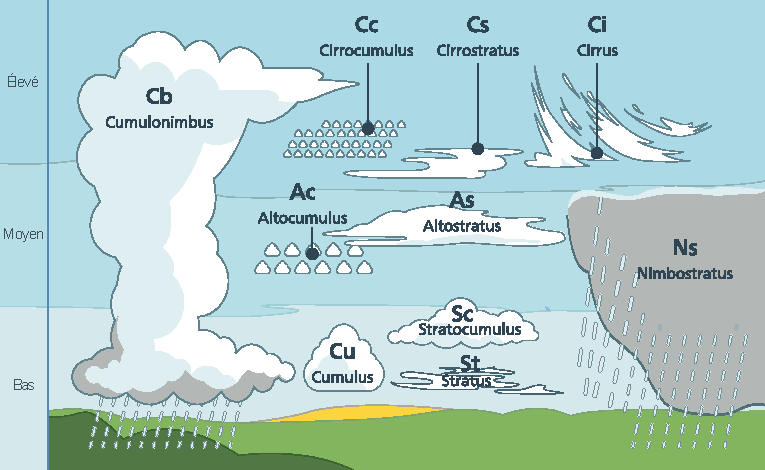
\includegraphics[width=0.75\textwidth]{03-Meteo/img/nuages.pdf}
    \legende{Répartition des types de nuages dans la troposhère}{img:nuages}
    \end{figure}	
		\section{Les vents}
		\section{Les masses d'air et les fronts}
		\section{Les phénomènes dangereux pour le vol}
	
	\chapter{Aérodynamique, aérostatique et principes du vol}
	\label{aerodynamique}
		\section{La sustentation et l'aile}



		\section{Étude du vol stabilisé}
	\subsection{Vol plané}
	
	\subsection{Vol stabilisé}
		\section{L'aérostation}
	\subsection{Principe généraux}
		\section{Le vol spatial}
	\subsection{Principe généraux}
	
	\chapter{Histoire et culture de l'aéronautique et du spatial}
	\label{histoire}
		\section{Du mythe à la réalité}
		\section{Des précurseurs aux pionniers}
		\section{Les enjeux militaires et les évolutions de l'aéronautique et du spatial}
		\section{Les enjeux économiques et les évolutions de l'aéronautique et du spatial}
		
	\appendix
	\chapter{Fiches pratiques}
	\section{Tableau des unités usuelles en aviation}	
	
	\begin{longtable}{
	|>{\centering}m{1.8cm}
	|>{\centering}m{2.8cm}
	|c
	|>{\centering}m{3.2cm}
	|c
	|}

 \hline
 Grandeur & Unité aéronautique & Abbrev. &  Valeur exacte & Valeur approchée\\
 \hline
 %\endfirsthead
 Hauteur Altitude & pieds \anglais{feet}\footnote{Le pied est utilisé pour l'altitude en aéronautique partout dans le monde sauf en Russie, qui utilise le mètre. Les vélivoles (planeurs) utilisent également le mètre pour l'altitude.} & ft & 1~ft = 0,3048~m & 1~m $\approx$ 3~pieds \\
 \hline
 Vitesse verticale & pieds/minute & ft/min & 1000~ft/min = 5,08~m/s & 1000~ft/min $\approx$ 5~m/s \\
 \hline
 Distance & mille nautique \anglais{nautical mile} & NM & 1~NM = 1852~m & \\
 \hline
 Vitesse & nœud \anglais{knot} & kt & 1~kt~=~1~NM/h 1~kt~=~1,852~km/h 1~kt~=~0,514~m/s & 1~kt~$\approx$~2~km/h\\
 \hline
 
 \caption{Tableau récapitulatif des unités utilisées en aéronautique}
 \end{longtable}
	
	\section{L'alphabet radio international}
	\begin{center}
	\begin{longtable}{|L{0.5cm}|L{3.5cm}||L{0.5cm}|L{3.5cm}||L{0.5cm}|L{3.5cm}|}
		\hline
			A & Alpha & 				J & Juliett &			S & Sierra \tabularnewline
		\hline
			B & Bravo & 				K & Kilo &				T & Tango \tabularnewline
		\hline
			C & Charlie & 			L & Lima &				U & Uniform \tabularnewline
		\hline
			D & Delta & 				M & Mike &				V & Victor \tabularnewline	
		\hline
			E & Echo & 				N & November &			W & Wiskey \tabularnewline
		\hline
			F & Fox-trot & 			O & Oscar &				X & X-Ray \tabularnewline
		\hline
			G & Golf & 				P & Papa &				Y & Yankee \tabularnewline
		\hline
			H & Hotel & 				Q & Quebec &				Z & Zoulou \tabularnewline
		\hline
			I & India & 				R & Romeo &				0 & Zéro \anglais{zero} \tabularnewline
		\hline
			1 & Unité \anglais{one} & 2 & Deux \anglais{two}   & 3 & Trois \anglais{three} \tabularnewline
		\hline
			4 & Quatre \anglais{four} & 5 & Cinq \anglais{five} &	6 & Six \anglais{six} \tabularnewline
		\hline
			7 & Sept \anglais{sevent} & 	8 & Huit \anglais{eight} & 9 & Neuf \anglais{nine\footnote{Prononcé 'niner'}} \tabularnewline
		\hline
	\caption{L'alphabet radio international}
	\end{longtable}
\end{center}
	
	\chapter{Des questions pour pousser la réflexion !}
	\section{Étude des aéronefs}
	\question{"Le parachute est-il un aéronef ? Pourquoi ?" (en parlant du parachute coupole)}
	
	\chapter{Extraits de documents}
	\section{Extraits de cartes aéronautique}
\subsection{Carte IGN OACI 1/500 000 - région Bordeaux}
\hyperlink{ignOaciBordeaux.1}{Voir la carte IGN OACI de Bordeaux} (Source : \cite{img:ignOaciBordeaux})

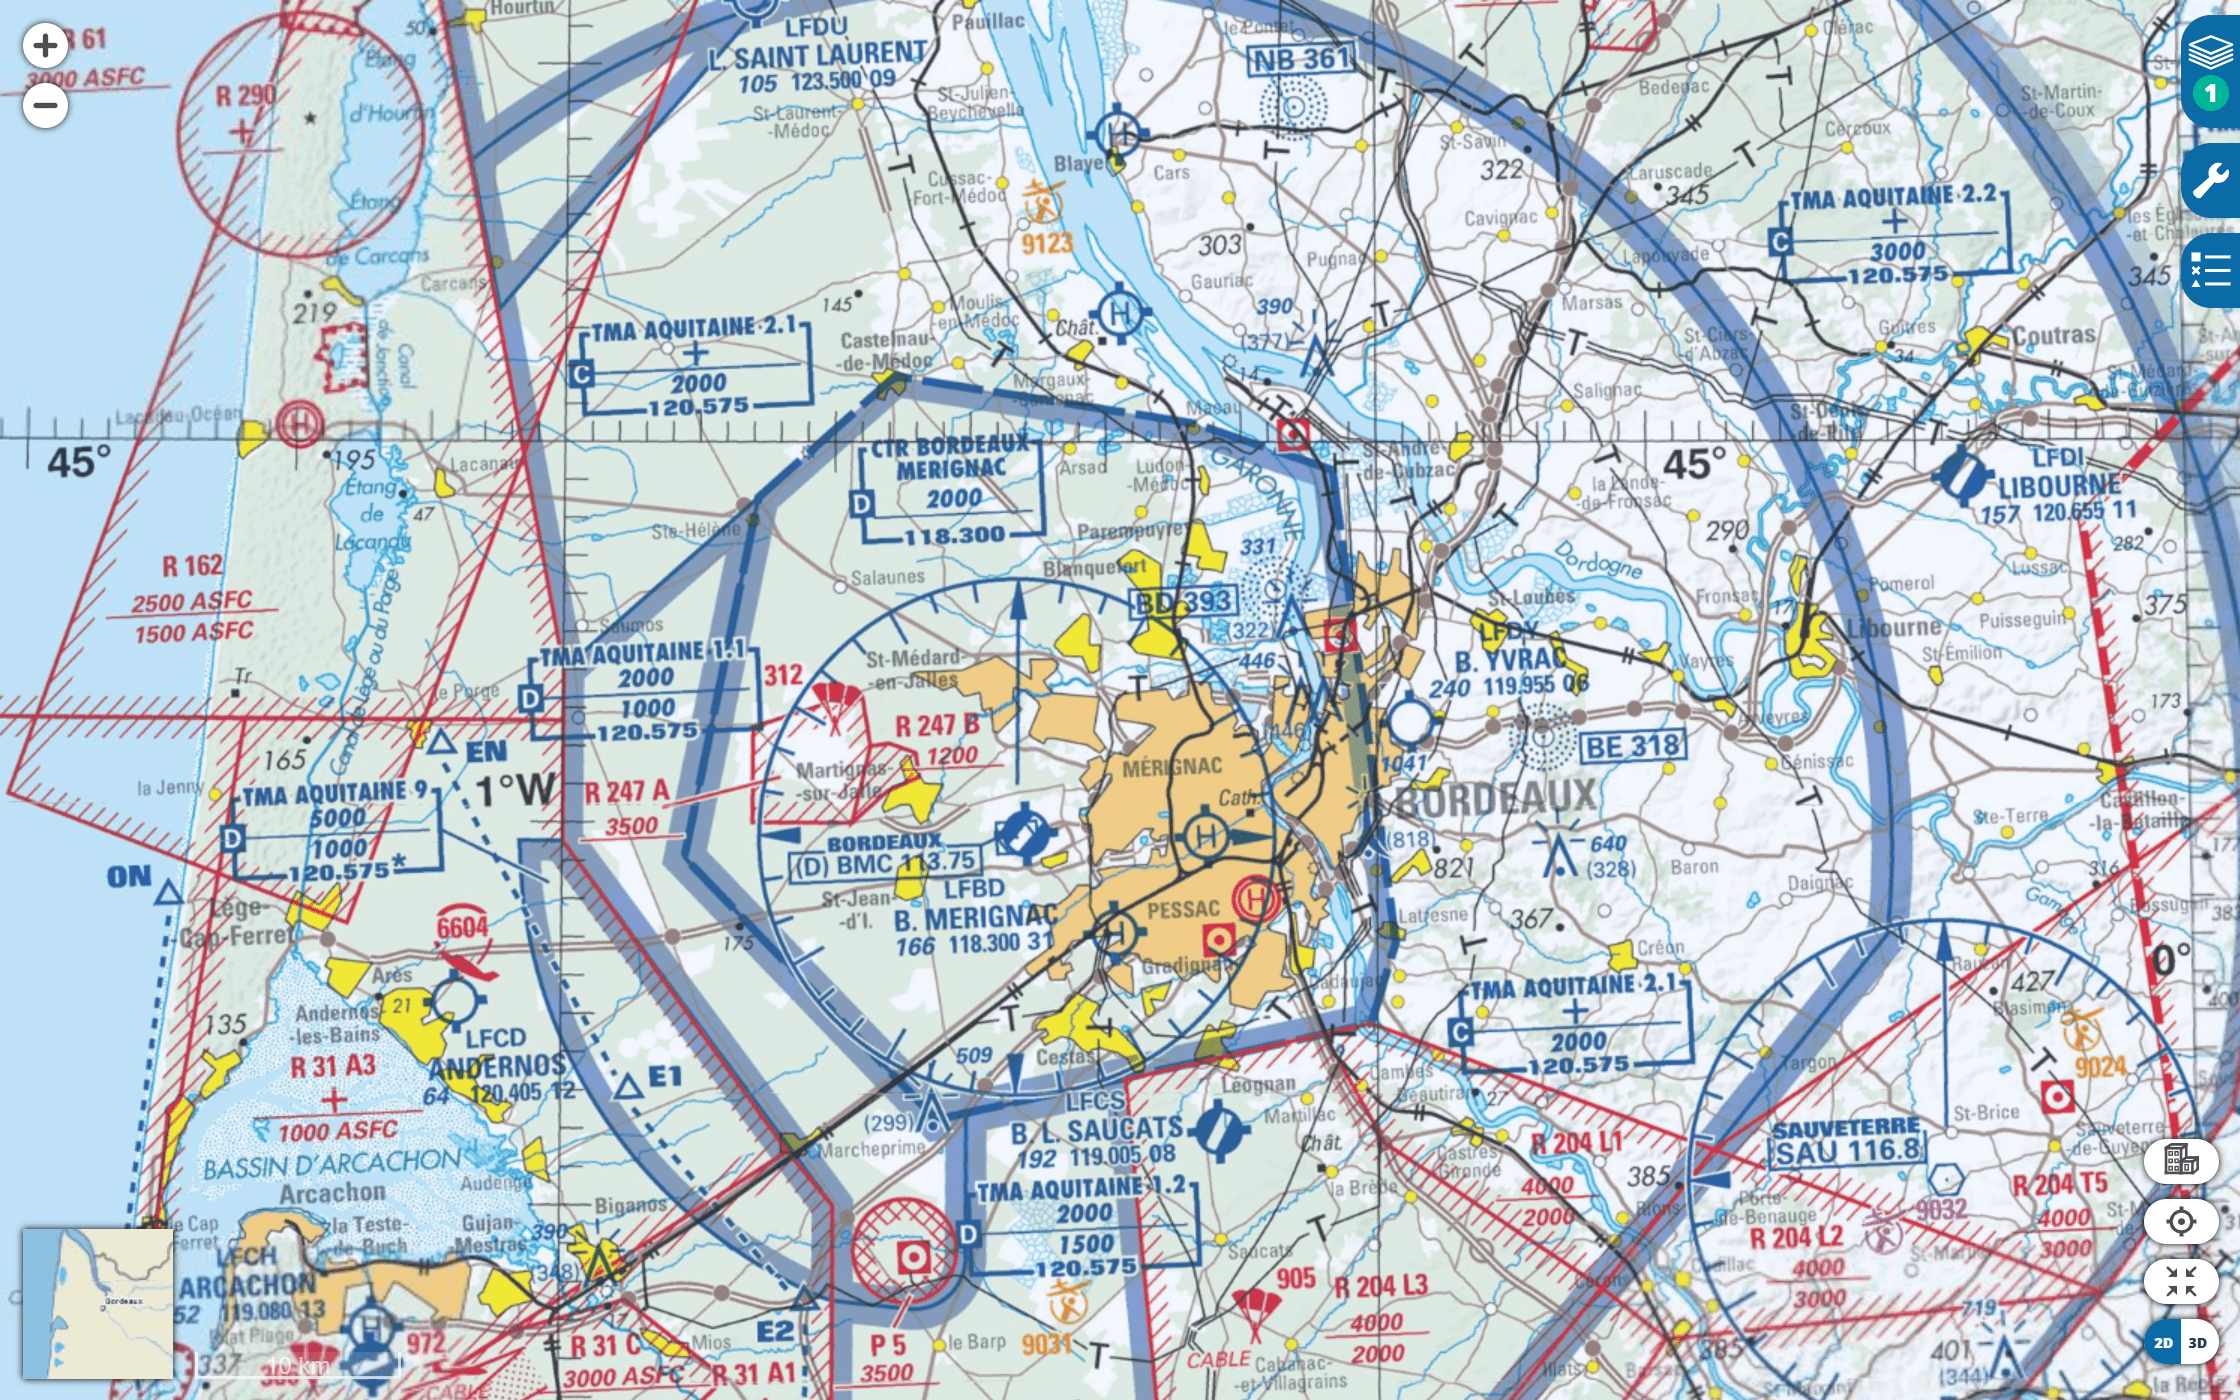
\includepdf[landscape=true, 
link=true, 
linkname=ignOaciBordeaux,
addtolist={1,figure,{Extrait de la carte IGN OACI 2024, secteur Bordeaux (Source : \cite{img:ignOaciBordeaux})},ignOaciBdx}]{./Annexes/img/ignOaciBordeaux.png}


	
%\chapter{Table des matières}
	\setcounter{tocdepth}{5}
	\tableofcontents
	
	\listoffigures
	
	\listoftables
	
	\printglossaries

%\chapter{Bibliographie}
	\nocite{*}
	%\bibliographystyle{unsrt-fr}
	%\bibliography{1-EtudeAeronefs/biblio}
	%\printbibliography
	%\bibliography{1-EtudeAeronefs/biblio}
	%\printbibliography[heading=bibintoc,title={Bibliographie}]
	
	\chapter*{Bibliographie}
	\addcontentsline{toc}{chapter}{Bibliographie}
	\printbibliography[heading=subbibintoc,title={Livres},type=book]
	\printbibliography[heading=subbibintoc,title={Ressources en ligne},type=online]
	\printbibliography[heading=subbibintoc,title={Images},type=misc]
	\printbibliography[heading=subbibintoc,title={Logiciels},type=proceedings]
	
\end{document}